\documentclass[11pt, letterpaper]{article}

% Fonts and Encoding
\usepackage[utf8]{inputenc}
\usepackage[T1]{fontenc}
\usepackage{lmodern} % High-quality Latin Modern vector font

% Math and Symbols
\usepackage{amsmath, amssymb, amsthm, amsfonts, mathrsfs, mathtools}

% Layout and Geometry
\usepackage{geometry}
\geometry{letterpaper, margin=1in}
\setlength{\parindent}{0pt}
\setlength{\parskip}{0.6em}

% Formatting and Graphics
\usepackage{graphicx, xcolor, enumitem, booktabs, array, tabularx}

% TikZ for Illustrations
\usepackage{tikz}
\usetikzlibrary{arrows.meta, positioning, shapes.geometric, calc, backgrounds, matrix}

% Clickable Links and TOC
\usepackage{hyperref}
\hypersetup{
    colorlinks=true,
    linkcolor=blue,
    filecolor=magenta,      
    urlcolor=cyan,
    pdftitle={Denumerable Sets: Rigorous Foundations, Proofs, and Quantitative Applications},
}

% Theorem Environments
\newtheorem{theorem}{Theorem}[section]
\newtheorem{lemma}[theorem]{Lemma}
\newtheorem{proposition}[theorem]{Proposition}
\newtheorem{corollary}[theorem]{Corollary}
\theoremstyle{definition}
\newtheorem{definition}{Definition}[section]
\newtheorem{axiom}{Axiom}[section]
\newtheorem{example}{Example}[section]
\theoremstyle{remark}
\newtheorem{remark}{Remark}[section]

% Custom Commands (Enforced standard notation)
\newcommand{\R}{\mathbb{R}}
\newcommand{\N}{\mathbb{N}}
\newcommand{\Z}{\mathbb{Z}}
\newcommand{\Q}{\mathbb{Q}}
\newcommand{\E}{\mathbb{E}}
\newcommand{\Prob}{\mathbb{P}}
\newcommand{\F}{\mathcal{F}}

\title{\textbf{Denumerable Sets: Rigorous Foundations, Complete Proofs, and Quantitative Applications}}
\author{Tashfeen Omran}
\date{\today}

\begin{document}

\maketitle
\tableofcontents
\newpage

% ============================================================================
% PART 1: COMPREHENSIVE INTRODUCTION, CONTEXT, AND PREREQUISITES
% ============================================================================
\section{Comprehensive Introduction, Context, and Prerequisites}

\subsection{Core Concepts and Axioms}

The mathematical study of infinite sets begins by replacing naive intuition about ``size'' with a rigorous set-theoretic criterion grounded in bijective mappings. Throughout this chapter, we adopt the canonical convention that the set of natural numbers is the set of positive integers, $\mathbb{N} = \{1, 2, 3, \dots\}$, and recall that two sets $A$ and $B$ have the same cardinality, written $|A| = |B|$ (or are \emph{numerically equivalent}), if and only if there exists a bijective function $f : A \to B$.

\begin{definition}[Denumerable Set]
A set $A$ is called \emph{denumerable} if $|A| = |\mathbb{N}|$; that is, there exists a bijective (both one-to-one and onto) function $f : \mathbb{N} \to A$.
\end{definition}

When $f : \mathbb{N} \to A$ is a bijection, the function can be written as a set of ordered pairs $f = \{(1, f(1)), (2, f(2)), (3, f(3)), \dots\}$. Writing $a_i = f(i)$ for each $i \in \mathbb{N}$, we obtain a sequential enumeration $A = \{a_1, a_2, a_3, \dots\}$ in which every element of $A$ appears \emph{exactly once} (i.e., $a_i \neq a_j$ whenever $i \neq j$). Conversely, if the elements of $A$ can be listed without repetition as a sequence $a_1, a_2, a_3, \dots$, then the function $g : \mathbb{N} \to A$ defined by $g(n) = a_n$ is bijective. Hence, a set $A$ is denumerable if and only if its elements can be arranged into an infinite sequence with no repetitions.

\begin{definition}[Countable and Uncountable Sets]
A set $A$ is called \emph{countable} if $A$ is either finite or denumerable. Thus, a \emph{countably infinite} set is precisely a denumerable set. A nonempty countable set can be written either as $A = \{a_1, a_2, \dots, a_n\}$ for some $n \in \mathbb{N}$ or as $A = \{a_1, a_2, a_3, \dots\}$. A set that is not countable is called \emph{uncountable}. Every uncountable set is necessarily infinite.
\end{definition}

Two foundational axioms and principles of arithmetic and set theory power virtually every rigorous proof concerning denumerable sets:

\begin{axiom}[Well-Ordering Principle]
Every nonempty subset $S \subseteq \mathbb{N}$ possesses a least element; that is, there exists $m \in S$ such that $m \le s$ for all $s \in S$.
\end{axiom}

\begin{axiom}[Equivalence Properties of Cardinality]
Numerical equivalence is an equivalence relation on any collection of sets:
\begin{enumerate}[label=(\roman*)]
    \item \emph{Reflexivity:} $|A| = |A|$ via the identity bijection $i_A : A \to A$.
    \item \emph{Symmetry:} If $|A| = |B|$ via a bijection $f : A \to B$, then $|B| = |A|$ via the inverse bijection $f^{-1} : B \to A$.
    \item \emph{Transitivity:} If $|A| = |B|$ via $f : A \to B$ and $|B| = |C|$ via $g : B \to C$, then $|A| = |C|$ via the composite bijection $g \circ f : A \to C$.
\end{enumerate}
\end{axiom}

We also utilize the standard multiple-set notation: for any $k \in \mathbb{N}$,
\[
k\mathbb{Z} = \{kn : n \in \mathbb{Z}\} \quad \text{and} \quad k\mathbb{N} = \{kn : n \in \mathbb{N}\}.
\]
In particular, $1\mathbb{Z} = \mathbb{Z}$, $1\mathbb{N} = \mathbb{N}$, and $2\mathbb{Z}$ denotes the set of all even integers.

\subsection{Intuition and Set-Theoretic Foundations}

For finite sets, Euclid's classical common notion---``the whole is greater than the part''---holds unconditionally: if $B \subsetneq A$ and $A$ is finite, then $|B| < |A|$. For infinite sets, this intuition breaks down dramatically. A denumerable set can be placed into exact one-to-one correspondence with a \emph{proper subset} of itself. For example, $\mathbb{N} \subsetneq \mathbb{Z}$, yet $|\mathbb{N}| = |\mathbb{Z}|$; likewise, $2\mathbb{Z} \subsetneq \mathbb{Z}$, yet $|2\mathbb{Z}| = |\mathbb{Z}|$.

Geometrically and algorithmically, you should envision a denumerable set $A$ as a collection of objects that can be placed onto an infinitely long numbered conveyor belt, with slots labeled $1, 2, 3, \dots$, such that:
\begin{itemize}
    \item Every slot holds at most one item (well-definedness of $f : \mathbb{N} \to A$).
    \item No item appears in two different slots (injectivity).
    \item Every element of $A$ eventually passes the inspection gate at some finite index $n \in \mathbb{N}$ (surjectivity).
\end{itemize}

This conveyor-belt perspective immediately clarifies why naive traversal strategies fail on two-dimensional infinite grids such as $\mathbb{N} \times \mathbb{N}$ or the fraction table for $\mathbb{Q}^+$. If one attempts to traverse an infinite grid \emph{row by row}, the first row never terminates; one exhausts all of $\mathbb{N}$ on Row $1$ alone and never reaches Row $2$. To ensure surjectivity, the enumeration path must visit finite shells that progressively sweep out the entire grid---most famously via Cantor's diagonal traversal, where pairs $(i, j)$ are grouped by the finite constant sum $i + j = c$ for $c = 2, 3, 4, \dots$. Because each diagonal $i + j = c$ contains only $c - 1$ entries, every single grid entry $(i, j)$ is guaranteed to be reached in finitely many steps.

\subsection{Historical Context and Motivation}

The paradoxes of infinite cardinality troubled mathematicians and philosophers for centuries. In his 1638 treatise \emph{Two New Sciences}, Galileo Galilei observed that the natural numbers $1, 2, 3, 4, \dots$ can be paired bijectively with the perfect squares $1, 4, 9, 16, \dots$ via $n \mapsto n^2$, despite the squares forming a seemingly sparse proper subset of $\mathbb{N}$. Unable to reconcile this with finite intuition, Galileo concluded that the relations ``less than,'' ``equal to,'' and ``greater than'' could not be meaningfully applied to infinite quantities.

Nearly two and a half centuries later, in the 1870s, Georg Cantor revolutionized the foundations of mathematics while studying uniqueness theorems for trigonometric (Fourier) series. Cantor realized that Galileo's phenomenon was not a logical defect, but rather the defining structural hallmark of infinite sets (later formalized by Richard Dedekind as \emph{Dedekind-infiniteness}). By demonstrating in 1874 that the integers $\mathbb{Z}$, the Cartesian product $\mathbb{N} \times \mathbb{N}$, and even the dense set of rational numbers $\mathbb{Q}$ all share the same smallest infinite cardinality $|\mathbb{N}|$ (denoted $\aleph_0$), Cantor established a rigorous arithmetic of infinity. This breakthrough laid the foundation for modern point-set topology, measure theory, Kolmogorov's axiomatic probability theory (which relies on \emph{countable additivity}), and theoretical computer science.

\subsection{Key Theorems, Lemmas, and Formulas}

The core results established in Section 11.2 form the analytical backbone for all subsequent proofs and applications:

\begin{theorem}[Result 11.3: Denumerability of $\mathbb{Z}$]
The set $\mathbb{Z}$ of all integers is denumerable. Explicitly, the function $f : \mathbb{N} \to \mathbb{Z}$ given by
\[
f(n) = \frac{1 + (-1)^n (2n - 1)}{4}
\]
maps $1 \mapsto 0$, $2 \mapsto 1$, $3 \mapsto -1$, $4 \mapsto 2$, $5 \mapsto -2, \dots$, and is a bijection.
\end{theorem}

\begin{theorem}[Theorem 11.4: Infinite Subsets of Denumerable Sets]
Every infinite subset of a denumerable set is denumerable.
\end{theorem}

\begin{corollary}[Result 11.5: Denumerability of $2\mathbb{Z}$ and $k\mathbb{Z}$]
The set $2\mathbb{Z}$ of even integers is denumerable. More generally, for every nonzero integer $k$, the set $k\mathbb{Z}$ is denumerable because $k\mathbb{Z}$ is an infinite subset of the denumerable set $\mathbb{Z}$.
\end{corollary}

\begin{theorem}[Result 11.6: Cartesian Product of Denumerable Sets]
If $A$ and $B$ are denumerable sets, then their Cartesian product $A \times B = \{(a, b) : a \in A,\ b \in B\}$ is denumerable.
\end{theorem}

\begin{theorem}[Result 11.7: Denumerability of $\mathbb{Q}^+$]
The set $\mathbb{Q}^+$ of positive rational numbers is denumerable.
\end{theorem}

\begin{theorem}[Result 11.8: Denumerability of $\mathbb{Q}$]
The set $\mathbb{Q}$ of all rational numbers is denumerable.
\end{theorem}

\subsection{Prerequisites}

To master denumerable sets and construct airtight proofs, the reader must be fluent in the following foundational concepts:
\begin{itemize}
    \item \textbf{Functions and Bijections:} Proving well-definedness, injectivity ($f(x_1) = f(x_2) \implies x_1 = x_2$), surjectivity ($\forall y \in B,\ \exists x \in A$ such that $f(x) = y$), inverses, and compositions of bijections.
    \item \textbf{Set Theory Operations:} Subsets, proper subsets, set differences ($A - B$), unions (finite and indexed infinite unions $\bigcup_{i=1}^{\infty} A_i$), pairwise disjointness, partitions of a set, and Cartesian products.
    \item \textbf{Proof Techniques:} Direct proof, proof by cases (especially parity cases: even vs.\ odd integers), proof by contradiction, mathematical induction, strong induction, and applications of the Well-Ordering Principle on $\mathbb{N}$.
    \item \textbf{Elementary Number Theory:} Parity arguments, irrationality of $\sqrt{2}$, unique factorization of positive integers into a power of $2$ times an odd integer, and basic properties of complex numbers.
\end{itemize}

% ============================================================================
% PART 2: DETAILED HOMEWORK SOLUTIONS
% ============================================================================
\section{Detailed Homework Solutions (Section 11.2 Exercises)}

Below are complete, rigorous solutions to every exercise in Section 11.2 (Exercises 11.3 through 11.19). Each original problem statement is reproduced verbatim prior to its proof.

% --- Exercise 11.3 ---
\subsection{Exercise 11.3}

\textbf{Original Problem:} Prove that if $A$ and $B$ are disjoint denumerable sets, then $A \cup B$ is denumerable.

\textbf{Proof Technique:} Direct Constructive Proof (via an explicit alternating bijection from $\mathbb{N}$ to $A \cup B$).

\begin{proof}
Assume that $A$ and $B$ are disjoint denumerable sets, so $A \cap B = \emptyset$, $|A| = |\mathbb{N}|$, and $|B| = |\mathbb{N}|$. By the definition of a denumerable set, we may list the elements of $A$ and $B$ without repetition as
\[
A = \{a_1, a_2, a_3, \dots\} \quad \text{and} \quad B = \{b_1, b_2, b_3, \dots\},
\]
where $a_i \neq a_j$ and $b_i \neq b_j$ whenever $i \neq j$. Furthermore, since $A \cap B = \emptyset$, we have $a_i \neq b_j$ for all $i, j \in \mathbb{N}$.

Define a function $f : \mathbb{N} \to A \cup B$ by interleaving the elements of $A$ and $B$ according to the parity of $n \in \mathbb{N}$:
\[
f(n) = \begin{cases}
a_{(n+1)/2} & \text{if } n \text{ is odd}, \\[4pt]
b_{n/2} & \text{if } n \text{ is even}.
\end{cases}
\]
We verify that $f$ is well-defined, injective, and surjective.

\emph{Well-definedness:} If $n \in \mathbb{N}$ is odd, then $n = 2k - 1$ for a unique $k \in \mathbb{N}$, so $(n+1)/2 = k \in \mathbb{N}$ and $f(n) = a_k \in A \subseteq A \cup B$. If $n \in \mathbb{N}$ is even, then $n = 2k$ for a unique $k \in \mathbb{N}$, so $n/2 = k \in \mathbb{N}$ and $f(n) = b_k \in B \subseteq A \cup B$. Thus $f$ is well-defined.

\emph{Injectivity:} Suppose $f(n_1) = f(n_2)$ for some $n_1, n_2 \in \mathbb{N}$. We claim $n_1$ and $n_2$ must have the same parity. Suppose for contradiction that one is odd and the other is even; without loss of generality, let $n_1$ be odd and $n_2$ be even. Then $f(n_1) = a_{(n_1+1)/2} \in A$ while $f(n_2) = b_{n_2/2} \in B$, which implies $f(n_1) \in A \cap B$, contradicting $A \cap B = \emptyset$. Therefore, $n_1$ and $n_2$ have the same parity.
\begin{itemize}
    \item \emph{Case 1 ($n_1, n_2$ both odd):} Then $a_{(n_1+1)/2} = a_{(n_2+1)/2}$. Because the elements of $A$ are listed without repetition, $(n_1 + 1)/2 = (n_2 + 1)/2$, which yields $n_1 = n_2$.
    \item \emph{Case 2 ($n_1, n_2$ both even):} Then $b_{n_1/2} = b_{n_2/2}$. Because the elements of $B$ are listed without repetition, $n_1/2 = n_2/2$, which yields $n_1 = n_2$.
\end{itemize}
Hence $f$ is one-to-one.

\emph{Surjectivity:} Let $x \in A \cup B$.
\begin{itemize}
    \item If $x \in A$, then $x = a_k$ for some $k \in \mathbb{N}$. Choose $n = 2k - 1 \in \mathbb{N}$. Then $n$ is odd and $f(2k - 1) = a_{((2k-1)+1)/2} = a_k = x$.
    \item If $x \in B$, then $x = b_k$ for some $k \in \mathbb{N}$. Choose $n = 2k \in \mathbb{N}$. Then $n$ is even and $f(2k) = b_{(2k)/2} = b_k = x$.
\end{itemize}
Hence $f$ is onto.

Since $f : \mathbb{N} \to A \cup B$ is bijective, $|A \cup B| = |\mathbb{N}|$, and therefore $A \cup B$ is denumerable.
\end{proof}

% --- Exercise 11.4 ---
\subsection{Exercise 11.4}

\textbf{Original Problem:} Let $\mathbb{R}^+$ denote the set of positive real numbers and let $A$ and $B$ be denumerable subsets of $\mathbb{R}^+$. Define $C = \{x \in \mathbb{R} : -x \in B\}$. Show that $A \cup C$ is denumerable.

\textbf{Proof Technique:} Direct Proof (establishing bijectivity between $B$ and $C$, verifying disjointness of $A$ and $C$, and applying Exercise 11.3).

\begin{proof}
First, we show that $C$ is denumerable. Define the function $g : B \to C$ by $g(b) = -b$ for all $b \in B$.
\begin{itemize}
    \item \emph{Well-definedness:} For any $b \in B$, we have $-(-b) = b \in B$, so by definition of $C$, $-b \in C$.
    \item \emph{Injectivity:} If $g(b_1) = g(b_2)$ for $b_1, b_2 \in B$, then $-b_1 = -b_2$, which implies $b_1 = b_2$.
    \item \emph{Surjectivity:} Let $x \in C$. By the definition of $C$, $-x \in B$. Setting $b = -x \in B$, we obtain $g(b) = -(-x) = x$.
\end{itemize}
Therefore, $g : B \to C$ is bijective, so $|C| = |B|$. Since $B$ is denumerable, $|B| = |\mathbb{N}|$. By transitivity of numerical equivalence, $|C| = |\mathbb{N}|$, meaning $C$ is denumerable.

Next, we verify that $A$ and $C$ are disjoint. Suppose for the sake of contradiction that there exists $x \in A \cap C$. Since $x \in A$ and $A \subseteq \mathbb{R}^+$, we have $x > 0$. On the other hand, since $x \in C$, we have $-x \in B \subseteq \mathbb{R}^+$, so $-x > 0$, which implies $x < 0$. This contradicts $x > 0$. Consequently, $A \cap C = \emptyset$.

Since $A$ and $C$ are disjoint denumerable sets, it follows directly from Exercise 11.3 that $A \cup C$ is denumerable.
\end{proof}

% --- Exercise 11.5 ---
\subsection{Exercise 11.5}

\textbf{Original Problem:} Prove that $|\mathbb{Z}| = |\mathbb{Z} - \{2\}|$.

\textbf{Proof Technique:} Direct Constructive Proof (exhibition of an explicit bijection $f : \mathbb{Z} \to \mathbb{Z} - \{2\}$, followed by a remark on an alternative Theorem 11.4 proof).

\begin{proof}
Define a function $f : \mathbb{Z} \to \mathbb{Z} - \{2\}$ by shifting all integers greater than or equal to $2$ upward by $1$:
\[
f(n) = \begin{cases}
n & \text{if } n < 2, \\[4pt]
n + 1 & \text{if } n \ge 2.
\end{cases}
\]
We prove that $f$ is well-defined, injective, and surjective.

\emph{Well-definedness:} If $n < 2$, then $f(n) = n < 2$, so $f(n) \neq 2$. If $n \ge 2$, then $f(n) = n + 1 \ge 3 > 2$, so $f(n) \neq 2$. In both cases, $f(n) \in \mathbb{Z} - \{2\}$.

\emph{Injectivity:} Suppose $f(n_1) = f(n_2)$ for $n_1, n_2 \in \mathbb{Z}$. Note that if $n < 2$, then $f(n) < 2$; if $n \ge 2$, then $f(n) \ge 3$. Thus it is impossible for one of $n_1, n_2$ to satisfy $n < 2$ and the other to satisfy $n \ge 2$.
\begin{itemize}
    \item \emph{Case 1 ($n_1 < 2$ and $n_2 < 2$):} Then $n_1 = f(n_1) = f(n_2) = n_2$.
    \item \emph{Case 2 ($n_1 \ge 2$ and $n_2 \ge 2$):} Then $n_1 + 1 = f(n_1) = f(n_2) = n_2 + 1$, so $n_1 = n_2$.
\end{itemize}
Hence $f$ is one-to-one.

\emph{Surjectivity:} Let $y \in \mathbb{Z} - \{2\}$. Since $y \in \mathbb{Z}$ and $y \neq 2$, either $y < 2$ or $y \ge 3$.
\begin{itemize}
    \item If $y < 2$, let $n = y \in \mathbb{Z}$. Then $n < 2$ and $f(n) = y$.
    \item If $y \ge 3$, let $n = y - 1 \in \mathbb{Z}$. Then $n \ge 2$ and $f(n) = (y - 1) + 1 = y$.
\end{itemize}
Hence $f$ is onto.

Because $f : \mathbb{Z} \to \mathbb{Z} - \{2\}$ is bijective, we conclude that $|\mathbb{Z}| = |\mathbb{Z} - \{2\}|$.
\end{proof}

\begin{remark}
Alternatively, by Result 11.3, $\mathbb{Z}$ is denumerable. Since $\mathbb{Z} - \{2\}$ is an infinite subset of $\mathbb{Z}$ (it contains $\{3, 4, 5, \dots\}$), Theorem 11.4 implies that $\mathbb{Z} - \{2\}$ is denumerable. By transitivity of numerical equivalence, $|\mathbb{Z}| = |\mathbb{N}| = |\mathbb{Z} - \{2\}|$.
\end{remark}

% --- Exercise 11.6 ---
\subsection{Exercise 11.6}

\textbf{Original Problem:}
\begin{enumerate}[label=(\alph*)]
    \item Prove that the function $f : \mathbb{R} - \{1\} \to \mathbb{R} - \{2\}$ defined by $f(x) = \dfrac{2x}{x - 1}$ is bijective.
    \item Explain why $|\mathbb{R} - \{1\}| = |\mathbb{R} - \{2\}|$.
\end{enumerate}

\textbf{Proof Technique:} Direct Proof (algebraic verification of well-definedness, injectivity, and surjectivity, followed by direct application of the definition of numerical equivalence).

\begin{proof}
\textbf{(a)} We verify that $f : \mathbb{R} - \{1\} \to \mathbb{R} - \{2\}$ is well-defined, one-to-one, and onto.

\emph{Well-definedness:} For every $x \in \mathbb{R} - \{1\}$, we have $x - 1 \neq 0$, so $f(x) = \frac{2x}{x-1} \in \mathbb{R}$ is defined. Moreover, $f(x) \neq 2$; indeed, if $\frac{2x}{x-1} = 2$, multiplying by $x - 1 \neq 0$ would give $2x = 2x - 2$, or $0 = -2$, a contradiction. Thus $f(x) \in \mathbb{R} - \{2\}$ for all $x \in \mathbb{R} - \{1\}$.

\emph{Injectivity:} Suppose $f(x_1) = f(x_2)$ for $x_1, x_2 \in \mathbb{R} - \{1\}$. Then
\[
\frac{2x_1}{x_1 - 1} = \frac{2x_2}{x_2 - 1}.
\]
Multiplying both sides by $(x_1 - 1)(x_2 - 1) \neq 0$ gives
\begin{align*}
2x_1(x_2 - 1) &= 2x_2(x_1 - 1) \\
2x_1 x_2 - 2x_1 &= 2x_1 x_2 - 2x_2 \\
-2x_1 &= -2x_2 \\
x_1 &= x_2.
\end{align*}
Thus $f$ is one-to-one.

\emph{Surjectivity:} Let $y \in \mathbb{R} - \{2\}$ be arbitrary. Since $y \neq 2$, we have $y - 2 \neq 0$. Define
\[
x = \frac{y}{y - 2} \in \mathbb{R}.
\]
We verify that $x$ belongs to the domain $\mathbb{R} - \{1\}$: if $\frac{y}{y-2} = 1$, then $y = y - 2$, giving $0 = -2$, a contradiction. Hence $x \in \mathbb{R} - \{1\}$. Evaluating $f(x)$, we obtain
\[
f(x) = \frac{2\left(\dfrac{y}{y - 2}\right)}{\dfrac{y}{y - 2} - 1} = \frac{\dfrac{2y}{y - 2}}{\dfrac{y - (y - 2)}{y - 2}} = \frac{2y}{2} = y.
\]
Hence $f$ is onto. Since $f$ is both one-to-one and onto, $f$ is bijective.

\textbf{(b)} By definition, two sets $A$ and $B$ have the same cardinality, $|A| = |B|$, if and only if there exists a bijective function from $A$ to $B$. Since part (a) established that $f : \mathbb{R} - \{1\} \to \mathbb{R} - \{2\}$ is a bijection, it follows immediately by definition that $|\mathbb{R} - \{1\}| = |\mathbb{R} - \{2\}|$.
\end{proof}

% --- Exercise 11.7 ---
\subsection{Exercise 11.7}

\textbf{Original Problem:} Let
\[
S = \left\{ x \in \mathbb{R} : x = \frac{n^2 + \sqrt{2}}{n},\ n \in \mathbb{N} \right\}.
\]
Define $f : \mathbb{N} \to S$ by $f(n) = \dfrac{n^2 + \sqrt{2}}{n}$.
\begin{enumerate}[label=(\alph*)]
    \item List three elements that belong to $S$.
    \item Show that $f$ is one-to-one.
    \item Show that $f$ is onto.
    \item Is $S$ denumerable? Explain.
\end{enumerate}

\textbf{Proof Technique:} Direct Evaluation for (a), Algebraic Proof with Irrationality/Integrality Contradiction for (b), Direct Proof from Set Definition for (c), and Application of the Definition of Denumerable Sets for (d).

\begin{proof}
\textbf{(a)} Evaluating $f(n)$ at $n = 1, 2, 3 \in \mathbb{N}$, three elements of $S$ are:
\[
f(1) = \frac{1^2 + \sqrt{2}}{1} = 1 + \sqrt{2}, \qquad
f(2) = \frac{2^2 + \sqrt{2}}{2} = \frac{4 + \sqrt{2}}{2}, \qquad
f(3) = \frac{3^2 + \sqrt{2}}{3} = \frac{9 + \sqrt{2}}{3}.
\]

\textbf{(b)} Suppose $f(m) = f(n)$ for some $m, n \in \mathbb{N}$. Then
\[
\frac{m^2 + \sqrt{2}}{m} = \frac{n^2 + \sqrt{2}}{n} \implies m + \frac{\sqrt{2}}{m} = n + \frac{\sqrt{2}}{n}.
\]
Rearranging terms yields
\begin{align*}
m - n &= \frac{\sqrt{2}}{n} - \frac{\sqrt{2}}{m} = \sqrt{2}\left(\frac{m - n}{mn}\right) \\
(m - n)\left(1 - \frac{\sqrt{2}}{mn}\right) &= 0.
\end{align*}
By the zero-product property in $\mathbb{R}$, either $m - n = 0$ or $1 - \frac{\sqrt{2}}{mn} = 0$. If $1 - \frac{\sqrt{2}}{mn} = 0$, then $mn = \sqrt{2}$. However, since $m, n \in \mathbb{N}$, the product $mn$ is a positive integer (hence rational), whereas $\sqrt{2}$ is irrational (and indeed $1 < \sqrt{2} < 2$ contains no integer). This is a contradiction. Therefore $m - n = 0$, so $m = n$. Hence $f$ is one-to-one.

\textbf{(c)} Let $x \in S$ be arbitrary. By the defining set-builder specification of $S$, there exists $n \in \mathbb{N}$ such that
\[
x = \frac{n^2 + \sqrt{2}}{n}.
\]
For this $n \in \mathbb{N}$, we immediately have $f(n) = \frac{n^2 + \sqrt{2}}{n} = x$. Therefore, $f$ is onto.

\textbf{(d)} Yes, $S$ is denumerable. By parts (b) and (c), $f : \mathbb{N} \to S$ is both one-to-one and onto, hence bijective. By the definition of a denumerable set, the existence of a bijection $f : \mathbb{N} \to S$ implies $|S| = |\mathbb{N}|$, so $S$ is denumerable.
\end{proof}

% --- Exercise 11.8 ---
\subsection{Exercise 11.8}

\textbf{Original Problem:} Prove that the function $f : \mathbb{N} \to \mathbb{Z}$ defined in (11.1) by $f(n) = \dfrac{1 + (-1)^n (2n - 1)}{4}$ is bijective.

\textbf{Proof Technique:} Direct Proof by Parity Cases (even vs.\ odd natural numbers).

\begin{proof}
We first simplify $f(n)$ according to the parity of $n \in \mathbb{N}$, which simultaneously establishes that $f$ is well-defined into $\mathbb{Z}$:
\begin{itemize}
    \item If $n \in \mathbb{N}$ is \emph{even}, write $n = 2k$ for a unique $k \in \mathbb{N}$. Then $(-1)^{2k} = 1$, so
    \[
    f(2k) = \frac{1 + (1)(4k - 1)}{4} = \frac{4k}{4} = k \in \mathbb{Z}^+.
    \]
    \item If $n \in \mathbb{N}$ is \emph{odd}, write $n = 2k - 1$ for a unique $k \in \mathbb{N}$. Then $(-1)^{2k-1} = -1$, so
    \[
    f(2k - 1) = \frac{1 + (-1)\bigl(2(2k - 1) - 1\bigr)}{4} = \frac{1 - (4k - 3)}{4} = \frac{4 - 4k}{4} = 1 - k \in \mathbb{Z}_{\le 0}.
    \]
\end{itemize}
Observe that $f(n) \ge 1$ whenever $n$ is even, whereas $f(n) \le 0$ whenever $n$ is odd. In particular, $f(n) \in \mathbb{Z}$ for every $n \in \mathbb{N}$, so $f : \mathbb{N} \to \mathbb{Z}$ is well-defined.

\emph{Injectivity:} Suppose $f(a) = f(b)$ for some $a, b \in \mathbb{N}$. Because even inputs yield strictly positive outputs ($f(n) \ge 1$) and odd inputs yield non-positive outputs ($f(n) \le 0$), $a$ and $b$ must share the same parity.
\begin{itemize}
    \item \emph{Case 1 ($a$ and $b$ are both even):} Write $a = 2j$ and $b = 2k$ with $j, k \in \mathbb{N}$. Then $j = f(2j) = f(2k) = k$, so $a = 2j = 2k = b$.
    \item \emph{Case 2 ($a$ and $b$ are both odd):} Write $a = 2j - 1$ and $b = 2k - 1$ with $j, k \in \mathbb{N}$. Then $1 - j = f(2j - 1) = f(2k - 1) = 1 - k$, which gives $j = k$ and hence $a = 2j - 1 = 2k - 1 = b$.
\end{itemize}
Therefore, $f$ is one-to-one.

\emph{Surjectivity:} Let $z \in \mathbb{Z}$ be arbitrary. We consider two exhaustive cases:
\begin{itemize}
    \item \emph{Case 1 ($z \ge 1$):} Set $n = 2z$. Since $z \in \mathbb{N}$, $n \in \mathbb{N}$ is even, and $f(n) = f(2z) = z$.
    \item \emph{Case 2 ($z \le 0$):} Set $k = 1 - z$. Since $z \le 0$, we have $k \ge 1$, so $k \in \mathbb{N}$. Now let $n = 2k - 1 = 1 - 2z \in \mathbb{N}$. Then $n$ is odd, and
    \[
    f(n) = f(2k - 1) = 1 - k = 1 - (1 - z) = z.
    \]
\end{itemize}
Therefore, $f$ is onto. Since $f$ is both one-to-one and onto, $f : \mathbb{N} \to \mathbb{Z}$ is bijective.
\end{proof}

% --- Exercise 11.9 ---
\subsection{Exercise 11.9}

\textbf{Original Problem:} Show that every denumerable set $A$ can be partitioned into two denumerable subsets of $A$.

\textbf{Proof Technique:} Direct Constructive Proof (splitting the sequential enumeration of $A$ by odd and even indices).

\begin{proof}
Let $A$ be a denumerable set. By definition, there exists a bijection $f : \mathbb{N} \to A$, so we may list the distinct elements of $A$ as $A = \{a_1, a_2, a_3, \dots\}$, where $a_n = f(n)$ for each $n \in \mathbb{N}$ and $a_i \neq a_j$ whenever $i \neq j$.

Define two subsets of $A$ corresponding to the odd-indexed and even-indexed elements:
\[
A_1 = \{a_{2k - 1} : k \in \mathbb{N}\} = \{a_1, a_3, a_5, \dots\} \quad \text{and} \quad A_2 = \{a_{2k} : k \in \mathbb{N}\} = \{a_2, a_4, a_6, \dots\}.
\]
We verify that $\{A_1, A_2\}$ is a partition of $A$ into two denumerable subsets:
\begin{enumerate}[label=(\arabic*)]
    \item \emph{Both $A_1$ and $A_2$ are denumerable (hence nonempty):} Define $g_1 : \mathbb{N} \to A_1$ by $g_1(k) = a_{2k-1}$ and $g_2 : \mathbb{N} \to A_2$ by $g_2(k) = a_{2k}$. Both are surjective by the definitions of $A_1$ and $A_2$. For injectivity, if $g_1(j) = g_1(k)$, then $a_{2j-1} = a_{2k-1}$, which implies $2j - 1 = 2k - 1$ (since $f$ is injective) and hence $j = k$; identically, $g_2(j) = g_2(k) \implies a_{2j} = a_{2k} \implies 2j = 2k \implies j = k$. Thus $g_1$ and $g_2$ are bijections, so $A_1$ and $A_2$ are denumerable (and in particular, $A_1 \neq \emptyset$ and $A_2 \neq \emptyset$).
    \item \emph{Disjointness ($A_1 \cap A_2 = \emptyset$):} Suppose for contradiction that $x \in A_1 \cap A_2$. Then $x = a_{2j-1} = a_{2k}$ for some $j, k \in \mathbb{N}$. Since $f$ is injective, $2j - 1 = 2k$, which is impossible because an odd integer cannot equal an even integer. Hence $A_1 \cap A_2 = \emptyset$.
    \item \emph{Exhaustiveness ($A_1 \cup A_2 = A$):} Clearly $A_1 \cup A_2 \subseteq A$. Conversely, let $a \in A$. Then $a = a_n$ for some $n \in \mathbb{N}$. If $n$ is odd, then $n = 2k - 1$ for some $k \in \mathbb{N}$, so $a \in A_1$. If $n$ is even, then $n = 2k$ for some $k \in \mathbb{N}$, so $a \in A_2$. Hence $A \subseteq A_1 \cup A_2$, yielding $A_1 \cup A_2 = A$.
\end{enumerate}
Therefore, $\{A_1, A_2\}$ is a partition of $A$ into two denumerable subsets.
\end{proof}

% --- Exercise 11.10 ---
\subsection{Exercise 11.10}

\textbf{Original Problem:} Let $A$ be a denumerable set and let $B = \{x, y\}$. Prove that $A \times B$ is denumerable.

\textbf{Proof Technique:} Direct Proof (decomposing $A \times B$ into two disjoint denumerable slices and applying Exercise 11.3; we also verify the degenerate case $x = y$ for complete rigor).

\begin{proof}
Since $A$ is denumerable, write $A = \{a_1, a_2, a_3, \dots\}$ with $a_i \neq a_j$ for $i \neq j$. Note that in standard notation $B = \{x, y\}$ denotes a $2$-element set with $x \neq y$ (if $x = y$, then $B = \{x\}$, and $a \mapsto (a, x)$ is trivially a bijection from $A$ to $A \times B$, making $A \times B$ denumerable). Assuming $x \neq y$, write
\[
A \times B = (A \times \{x\}) \cup (A \times \{y\}).
\]
Let $S_1 = A \times \{x\}$ and $S_2 = A \times \{y\}$.
\begin{itemize}
    \item \emph{$S_1$ is denumerable:} Define $g_1 : A \to S_1$ by $g_1(a) = (a, x)$. If $g_1(a) = g_1(a')$, then $(a, x) = (a', x)$, so $a = a'$; hence $g_1$ is injective. Every element of $S_1$ has the form $(a, x) = g_1(a)$ for some $a \in A$; hence $g_1$ is surjective. Thus $|S_1| = |A| = |\mathbb{N}|$, so $S_1$ is denumerable.
    \item \emph{$S_2$ is denumerable:} Analogously, $g_2 : A \to S_2$ defined by $g_2(a) = (a, y)$ is bijective, so $|S_2| = |A| = |\mathbb{N}|$ and $S_2$ is denumerable.
    \item \emph{Disjointness:} If $(a, b) \in S_1 \cap S_2$, then $b = x$ and $b = y$, contradicting $x \neq y$. Thus $S_1 \cap S_2 = \emptyset$.
\end{itemize}
Since $S_1$ and $S_2$ are disjoint denumerable sets, Exercise 11.3 guarantees that $A \times B = S_1 \cup S_2$ is denumerable.
\end{proof}

% --- Exercise 11.11 ---
\subsection{Exercise 11.11}

\textbf{Original Problem:} Let $B$ be a denumerable set and let $A$ be a nonempty set of unspecified cardinality. If $f : A \to B$ is a one-to-one function, then what can be said about the cardinality of $A$? Explain.

\textbf{Proof Technique:} Direct Proof by Cases (restricting the codomain of $f$ to its range $f(A)$ and applying Theorem 11.4).

\begin{proof}
\textbf{Claim:} The set $A$ must be a \emph{nonempty countable set}; that is, $A$ is either finite (with $|A| \in \mathbb{N}$) or denumerable ($|A| = |\mathbb{N}|$).

\textbf{Explanation and Proof:} Let $R = f(A) = \{f(a) : a \in A\} \subseteq B$ denote the range (image) of $f$. Because $A \neq \emptyset$, $R$ is also nonempty. Define the codomain-restricted function $\tilde{f} : A \to R$ by $\tilde{f}(a) = f(a)$ for all $a \in A$.
\begin{itemize}
    \item Since $f$ is one-to-one, $\tilde{f}(a_1) = \tilde{f}(a_2) \implies f(a_1) = f(a_2) \implies a_1 = a_2$, so $\tilde{f}$ is one-to-one.
    \item By definition of the range $R = f(A)$, for every $y \in R$ there exists $a \in A$ such that $\tilde{f}(a) = f(a) = y$, so $\tilde{f}$ is onto.
\end{itemize}
Thus $\tilde{f} : A \to R$ is a bijection, which implies $|A| = |R|$.

Now, $R$ is a nonempty subset of the denumerable set $B$. There are exactly two possibilities for $R$:
\begin{itemize}
    \item \emph{Case 1 ($R$ is finite):} Since $|A| = |R|$ and $R \neq \emptyset$, $A$ is a nonempty finite set with $|A| = |R| = k$ for some $k \in \mathbb{N}$.
    \item \emph{Case 2 ($R$ is infinite):} Since $R$ is an infinite subset of the denumerable set $B$, Theorem 11.4 implies that $R$ is denumerable, i.e., $|R| = |\mathbb{N}|$. By transitivity of numerical equivalence, $|A| = |R| = |\mathbb{N}|$, so $A$ is denumerable.
\end{itemize}
In both cases, $A$ is a nonempty countable set (either finite or denumerable), and in particular $A$ cannot be uncountable. Note that both outcomes are achievable: for $B = \mathbb{N}$, the inclusion $A \hookrightarrow \mathbb{N}$ is injective both when $A = \{1, 2, 3\}$ (finite) and when $A = 2\mathbb{N}$ (denumerable).
\end{proof}

% --- Exercise 11.12 ---
\subsection{Exercise 11.12}

\textbf{Original Problem:} Prove that the set of all $2$-element subsets of $\mathbb{N}$ is denumerable.

\textbf{Proof Technique:} Direct Proof via Injection into $\mathbb{N} \times \mathbb{N}$, combined with Result 11.6 and Theorem 11.4.

\begin{proof}
Let $\mathcal{P}_2(\mathbb{N}) = \{\{a, b\} : a, b \in \mathbb{N},\ a \neq b\}$ denote the set of all $2$-element subsets of $\mathbb{N}$. Notice that every element $X \in \mathcal{P}_2(\mathbb{N})$ consists of two distinct natural numbers, so $X$ has a unique representation $X = \{a, b\}$ with $a < b$.

Define the function $g : \mathcal{P}_2(\mathbb{N}) \to \mathbb{N} \times \mathbb{N}$ by
\[
g(\{a, b\}) = (a, b), \quad \text{where } a < b.
\]
\begin{itemize}
    \item \emph{Well-definedness:} Because every $2$-element subset of $\mathbb{N}$ has a unique minimum element $a$ and unique maximum element $b$, the ordered pair $(a, b) \in \mathbb{N} \times \mathbb{N}$ is uniquely determined by the set $\{a, b\}$.
    \item \emph{Injectivity:} Suppose $g(\{a_1, b_1\}) = g(\{a_2, b_2\})$ with $a_1 < b_1$ and $a_2 < b_2$. Then $(a_1, b_1) = (a_2, b_2)$, which forces $a_1 = a_2$ and $b_1 = b_2$, and hence $\{a_1, b_1\} = \{a_2, b_2\}$.
\end{itemize}
Let $R = g(\mathcal{P}_2(\mathbb{N})) = \{(a, b) \in \mathbb{N} \times \mathbb{N} : a < b\}$. Restricting the codomain of $g$ to $R$ yields a bijection $\tilde{g} : \mathcal{P}_2(\mathbb{N}) \to R$, so $|\mathcal{P}_2(\mathbb{N})| = |R|$.

Since $\mathbb{N}$ is denumerable, Result 11.6 implies that $\mathbb{N} \times \mathbb{N}$ is denumerable. Moreover, $R \subseteq \mathbb{N} \times \mathbb{N}$ is an infinite set because it contains the infinite collection of distinct ordered pairs $\{(1, k) : k \in \mathbb{N},\ k \ge 2\}$. By Theorem 11.4, $R$ is denumerable, so $|R| = |\mathbb{N}|$. By transitivity of numerical equivalence, $|\mathcal{P}_2(\mathbb{N})| = |R| = |\mathbb{N}|$, proving that $\mathcal{P}_2(\mathbb{N})$ is denumerable.
\end{proof}

% --- Exercise 11.13 ---
\subsection{Exercise 11.13}

\textbf{Original Problem:} A \textbf{Gaussian integer} is a complex number of the form $a + bi$, where $a, b \in \mathbb{Z}$ and $i = \sqrt{-1}$. Show that the set $\mathcal{G}$ of Gaussian integers is denumerable.

\textbf{Proof Technique:} Direct Proof via Bijection with $\mathbb{Z} \times \mathbb{Z}$, combined with Result 11.3 and Result 11.6.

\begin{proof}
Recall that $\mathcal{G} = \{a + bi : a, b \in \mathbb{Z}\}$. Define a function $f : \mathbb{Z} \times \mathbb{Z} \to \mathcal{G}$ by
\[
f(a, b) = a + bi \quad \text{for all } (a, b) \in \mathbb{Z} \times \mathbb{Z}.
\]
We verify that $f$ is bijective:
\begin{itemize}
    \item \emph{Well-definedness:} For any $a, b \in \mathbb{Z}$, $a + bi \in \mathcal{G}$ by definition.
    \item \emph{Injectivity:} Suppose $f(a_1, b_1) = f(a_2, b_2)$ for $(a_1, b_1), (a_2, b_2) \in \mathbb{Z} \times \mathbb{Z}$. Then $a_1 + b_1 i = a_2 + b_2 i$. By the definition of equality of complex numbers (equating real and imaginary parts), $a_1 = a_2$ and $b_1 = b_2$, so $(a_1, b_1) = (a_2, b_2)$. Thus $f$ is one-to-one.
    \item \emph{Surjectivity:} Let $z \in \mathcal{G}$ be arbitrary. By definition of $\mathcal{G}$, there exist integers $a, b \in \mathbb{Z}$ such that $z = a + bi$. Then $(a, b) \in \mathbb{Z} \times \mathbb{Z}$ satisfies $f(a, b) = a + bi = z$. Thus $f$ is onto.
\end{itemize}
Hence $|\mathcal{G}| = |\mathbb{Z} \times \mathbb{Z}|$. By Result 11.3, $\mathbb{Z}$ is denumerable. By Result 11.6, the Cartesian product of two denumerable sets is denumerable, so $\mathbb{Z} \times \mathbb{Z}$ is denumerable, i.e., $|\mathbb{Z} \times \mathbb{Z}| = |\mathbb{N}|$. By transitivity of numerical equivalence, $|\mathcal{G}| = |\mathbb{N}|$, so the set $\mathcal{G}$ of Gaussian integers is denumerable.
\end{proof}

% --- Exercise 11.14 ---
\subsection{Exercise 11.14}

\textbf{Original Problem:} Prove that $S = \{(a, b) : a, b \in \mathbb{N} \text{ and } b \ge 2a\}$ is denumerable.

\textbf{Proof Technique:} Direct Proof via Theorem 11.4 and Result 11.6.

\begin{proof}
By definition, every element $(a, b) \in S$ has $a \in \mathbb{N}$ and $b \in \mathbb{N}$, so $S \subseteq \mathbb{N} \times \mathbb{N}$. Since $\mathbb{N}$ is denumerable, Result 11.6 implies that $\mathbb{N} \times \mathbb{N}$ is denumerable.

Next, we demonstrate that $S$ is infinite. Consider the subset
\[
T = \{(n, 2n) : n \in \mathbb{N}\}.
\]
For every $n \in \mathbb{N}$, both $n$ and $2n$ belong to $\mathbb{N}$ and satisfy $2n \ge 2n$, so $(n, 2n) \in S$; thus $T \subseteq S$. The map $h : \mathbb{N} \to T$ given by $h(n) = (n, 2n)$ is bijective (if $(n_1, 2n_1) = (n_2, 2n_2)$ then $n_1 = n_2$, and surjectivity is immediate by definition of $T$). Hence $T$ is denumerable, which implies $T$ is infinite. Because $T \subseteq S$, $S$ must also be infinite.

Therefore, $S$ is an infinite subset of the denumerable set $\mathbb{N} \times \mathbb{N}$. By Theorem 11.4, $S$ is denumerable.
\end{proof}

% --- Exercise 11.15 ---
\subsection{Exercise 11.15}

\textbf{Original Problem:} Let $S \subseteq \mathbb{N} \times \mathbb{N}$ be defined by $S = \{(i, j) : i \le j\}$. Show that $S$ is denumerable.

\textbf{Proof Technique:} Direct Proof via Theorem 11.4 and Result 11.6.

\begin{proof}
We are given that $S \subseteq \mathbb{N} \times \mathbb{N}$. Since $\mathbb{N}$ is denumerable, Result 11.6 establishes that $\mathbb{N} \times \mathbb{N}$ is denumerable.

We verify that $S$ is infinite. For every $j \in \mathbb{N}$, we have $1 \le j$, so the ordered pair $(1, j)$ belongs to $S$. Define $T = \{(1, j) : j \in \mathbb{N}\} \subseteq S$. The map $j \mapsto (1, j)$ is clearly a bijection from $\mathbb{N}$ onto $T$, so $T$ is denumerable and therefore infinite. Since $T \subseteq S$, it follows that $S$ is infinite.

As $S$ is an infinite subset of the denumerable set $\mathbb{N} \times \mathbb{N}$, Theorem 11.4 implies that $S$ is denumerable.
\end{proof}

% --- Exercise 11.16 ---
\subsection{Exercise 11.16}

\textbf{Original Problem:} Let $A_1, A_2, A_3, \dots$ be pairwise disjoint denumerable sets. Prove that $\bigcup_{i=1}^{\infty} A_i$ is denumerable.

\textbf{Proof Technique:} Direct Constructive Proof (establishing a bijection from $\mathbb{N} \times \mathbb{N}$ onto $\bigcup_{i=1}^{\infty} A_i$ and composing with a bijection $\mathbb{N} \to \mathbb{N} \times \mathbb{N}$ from Result 11.6).

\begin{proof}
For each $i \in \mathbb{N}$, since $A_i$ is denumerable, there exists a bijective function $g_i : \mathbb{N} \to A_i$, allowing us to write
\[
A_i = \{a_{i, 1}, a_{i, 2}, a_{i, 3}, \dots\},
\]
where $a_{i, j} = g_i(j)$ for each $j \in \mathbb{N}$, and $a_{i, j_1} \neq a_{i, j_2}$ whenever $j_1 \neq j_2$. Furthermore, because the sets $A_1, A_2, A_3, \dots$ are pairwise disjoint, we have $A_{i_1} \cap A_{i_2} = \emptyset$ whenever $i_1 \neq i_2$.

Define the function $h : \mathbb{N} \times \mathbb{N} \to \bigcup_{i=1}^{\infty} A_i$ by
\[
h(i, j) = a_{i, j} \quad \text{for all } (i, j) \in \mathbb{N} \times \mathbb{N}.
\]
We prove that $h$ is bijective:
\begin{itemize}
    \item \emph{Well-definedness:} For every $(i, j) \in \mathbb{N} \times \mathbb{N}$, $a_{i, j} = g_i(j) \in A_i \subseteq \bigcup_{k=1}^{\infty} A_k$.
    \item \emph{Injectivity:} Suppose $h(i_1, j_1) = h(i_2, j_2)$ for $(i_1, j_1), (i_2, j_2) \in \mathbb{N} \times \mathbb{N}$. Then $a_{i_1, j_1} = a_{i_2, j_2}$. Denote this common element by $x$. Then $x \in A_{i_1}$ and $x \in A_{i_2}$, so $x \in A_{i_1} \cap A_{i_2}$, meaning $A_{i_1} \cap A_{i_2} \neq \emptyset$. Since the family $\{A_i\}_{i \in \mathbb{N}}$ is pairwise disjoint, this forces $i_1 = i_2$. Substituting $i_2 = i_1$ gives $g_{i_1}(j_1) = a_{i_1, j_1} = a_{i_1, j_2} = g_{i_1}(j_2)$. Because $g_{i_1}$ is injective, we conclude $j_1 = j_2$. Therefore $(i_1, j_1) = (i_2, j_2)$, so $h$ is one-to-one.
    \item \emph{Surjectivity:} Let $x \in \bigcup_{i=1}^{\infty} A_i$ be arbitrary. By definition of the indexed union, there exists $i \in \mathbb{N}$ such that $x \in A_i$. Since $g_i : \mathbb{N} \to A_i$ is surjective, there exists $j \in \mathbb{N}$ such that $g_i(j) = x$, i.e., $a_{i, j} = x$. Thus $(i, j) \in \mathbb{N} \times \mathbb{N}$ satisfies $h(i, j) = x$, proving $h$ is onto.
\end{itemize}
Since $h : \mathbb{N} \times \mathbb{N} \to \bigcup_{i=1}^{\infty} A_i$ is bijective, we have $\left|\bigcup_{i=1}^{\infty} A_i\right| = |\mathbb{N} \times \mathbb{N}|$. By Result 11.6, $|\mathbb{N} \times \mathbb{N}| = |\mathbb{N}|$. By transitivity of numerical equivalence, $\left|\bigcup_{i=1}^{\infty} A_i\right| = |\mathbb{N}|$, and thus $\bigcup_{i=1}^{\infty} A_i$ is denumerable.
\end{proof}

% --- Exercise 11.17 ---
\subsection{Exercise 11.17}

\textbf{Original Problem:} Let $A = \{a_1, a_2, a_3, \dots\}$. Define $B = A - \{a_{n^2} : n \in \mathbb{N}\}$. Prove that $|A| = |B|$.

\textbf{Proof Technique:} Direct Proof via Theorem 11.4 (exhibiting an infinite subset of $B$ using strict inequalities between consecutive perfect squares).

\begin{proof}
Here $A = \{a_1, a_2, a_3, \dots\}$ is a denumerable set listed without repetition ($a_i \neq a_j$ for $i \neq j$), so $|A| = |\mathbb{N}|$. By construction, $B = A - \{a_{n^2} : n \in \mathbb{N}\}$ is a subset of $A$. By Theorem 11.4, to show that $B$ is denumerable (and hence $|B| = |\mathbb{N}| = |A|$), it suffices to prove that $B$ is infinite.

Consider the subset $C \subseteq A$ defined by
\[
C = \{a_{k^2 + 1} : k \in \mathbb{N}\}.
\]
We claim that $C \subseteq B$. For any $k \in \mathbb{N}$, since $k \ge 1$, we have $2k \ge 2 > 0$, and therefore
\[
k^2 < k^2 + 1 < k^2 + 2k + 1 = (k + 1)^2.
\]
Because $k^2 + 1$ lies strictly between the two consecutive perfect squares $k^2$ and $(k+1)^2$, there is no integer $n \in \mathbb{N}$ such that $n^2 = k^2 + 1$. Since the elements of $A$ are pairwise distinct ($a_i = a_j \iff i = j$), it follows that $a_{k^2 + 1} \notin \{a_{n^2} : n \in \mathbb{N}\}$. Hence $a_{k^2 + 1} \in B$ for every $k \in \mathbb{N}$, establishing $C \subseteq B$.

Moreover, the function $\phi : \mathbb{N} \to C$ defined by $\phi(k) = a_{k^2 + 1}$ is bijective: it is surjective by definition of $C$, and if $\phi(k_1) = \phi(k_2)$, then $a_{k_1^2 + 1} = a_{k_2^2 + 1} \implies k_1^2 + 1 = k_2^2 + 1 \implies k_1^2 = k_2^2 \implies k_1 = k_2$ (as $k_1, k_2 \in \mathbb{N}$). Thus $C$ is denumerable, hence infinite. Because $C \subseteq B$, $B$ is an infinite subset of the denumerable set $A$.

Applying Theorem 11.4, $B$ is denumerable, so $|B| = |\mathbb{N}|$. By transitivity of numerical equivalence, $|A| = |\mathbb{N}| = |B|$.
\end{proof}

% --- Exercise 11.18 ---
\subsection{Exercise 11.18}

\textbf{Original Problem:} A function $f : \mathbb{N} \times \mathbb{N} \to \mathbb{N}$ is defined by $f(m, n) = 2^{m-1}(2n - 1)$.
\begin{enumerate}[label=(\alph*)]
    \item Prove that $f$ is one-to-one and onto.
    \item Show that $\mathbb{N} \times \mathbb{N}$ is denumerable.
\end{enumerate}

\textbf{Proof Technique:} Parity Contradiction for Injectivity and Strong Mathematical Induction for Surjectivity in (a); Symmetry of Numerical Equivalence (Inverse Bijection) for (b).

\begin{proof}
\textbf{(a)} First observe that for all $m, n \in \mathbb{N}$, $m - 1 \ge 0$ implies $2^{m-1} \in \mathbb{N}$, and $n \ge 1$ implies $2n - 1 \in \mathbb{N}$, so $f(m, n) \in \mathbb{N}$ is well-defined.

\emph{Injectivity:} Suppose $f(m_1, n_1) = f(m_2, n_2)$ for $(m_1, n_1), (m_2, n_2) \in \mathbb{N} \times \mathbb{N}$. Then
\[
2^{m_1 - 1}(2n_1 - 1) = 2^{m_2 - 1}(2n_2 - 1).
\]
We claim that $m_1 = m_2$. Suppose for the sake of contradiction that $m_1 \neq m_2$. Without loss of generality, assume $m_1 > m_2$, so $m_1 - m_2 \ge 1$. Dividing both sides of the equation by $2^{m_2 - 1} > 0$ yields
\[
2^{m_1 - m_2}(2n_1 - 1) = 2n_2 - 1.
\]
Since $m_1 - m_2 \ge 1$, the integer $2^{m_1 - m_2}$ is even, making the left-hand side even. However, the right-hand side $2n_2 - 1$ is odd---a contradiction. Thus $m_1 = m_2$.

Substituting $m_1 = m_2$ back into the original equation and dividing by $2^{m_1 - 1} > 0$ gives
\[
2n_1 - 1 = 2n_2 - 1 \implies 2n_1 = 2n_2 \implies n_1 = n_2.
\]
Hence $(m_1, n_1) = (m_2, n_2)$, proving that $f$ is one-to-one.

\emph{Surjectivity:} We prove by Strong Mathematical Induction on $k \in \mathbb{N}$ that for every $k \in \mathbb{N}$, there exist $m, n \in \mathbb{N}$ such that $f(m, n) = 2^{m-1}(2n - 1) = k$.
\begin{itemize}
    \item \emph{Base Case ($k = 1$):} Choose $m = 1$ and $n = 1$. Then $(1, 1) \in \mathbb{N} \times \mathbb{N}$ and
    \[
    f(1, 1) = 2^{1-1}(2(1) - 1) = 2^0 \cdot 1 = 1.
    \]
    \item \emph{Strong Inductive Step:} Let $k \in \mathbb{N}$ be arbitrary, and assume that every integer $j$ satisfying $1 \le j \le k$ belongs to the image of $f$ (i.e., $j = f(m, n)$ for some $m, n \in \mathbb{N}$). We must show that $k + 1$ belongs to the image of $f$. We consider two cases according to the parity of $k + 1$:
    \begin{itemize}
        \item \emph{Case 1 ($k + 1$ is odd):} Then $k + 1 = 2n - 1$ for some $n \in \mathbb{N}$ (specifically, $n = \frac{k+2}{2} \in \mathbb{N}$). Choosing $m = 1$, we have $(1, n) \in \mathbb{N} \times \mathbb{N}$ and
        \[
        f(1, n) = 2^{1-1}(2n - 1) = 2n - 1 = k + 1.
        \]
        \item \emph{Case 2 ($k + 1$ is even):} Then $k + 1 = 2j$ for some integer $j = \frac{k+1}{2} \in \mathbb{N}$. Since $k \ge 1$, we have $1 \le j = \frac{k+1}{2} \le k$. By the strong inductive hypothesis, there exist $m_0, n_0 \in \mathbb{N}$ such that $j = 2^{m_0 - 1}(2n_0 - 1)$. Setting $m = m_0 + 1 \in \mathbb{N}$ and $n = n_0 \in \mathbb{N}$, we obtain
        \[
        f(m, n) = 2^{(m_0 + 1) - 1}(2n_0 - 1) = 2 \cdot 2^{m_0 - 1}(2n_0 - 1) = 2j = k + 1.
        \]
    \end{itemize}
\end{itemize}
By the Strong Principle of Mathematical Induction, every $k \in \mathbb{N}$ lies in the range of $f$; hence $f$ is onto.

\textbf{(b)} From part (a), $f : \mathbb{N} \times \mathbb{N} \to \mathbb{N}$ is bijective. Consequently, its inverse function $f^{-1} : \mathbb{N} \to \mathbb{N} \times \mathbb{N}$ exists and is also bijective. By the definition of a denumerable set, $|\mathbb{N} \times \mathbb{N}| = |\mathbb{N}|$, so $\mathbb{N} \times \mathbb{N}$ is denumerable.
\end{proof}

% --- Exercise 11.19 ---
\subsection{Exercise 11.19}

\textbf{Original Problem:} Prove that every denumerable set $A$ can be partitioned into a denumerable number of denumerable subsets of $A$.

\textbf{Proof Technique:} Direct Constructive Proof (composing a bijection $g : \mathbb{N} \to A$ with the explicit bijection $f : \mathbb{N} \times \mathbb{N} \to \mathbb{N}$ from Exercise 11.18 to index the partition blocks by row).

\begin{proof}
Let $A$ be a denumerable set. By definition, there exists a bijection $g : \mathbb{N} \to A$. By Exercise 11.18(a), the function $f : \mathbb{N} \times \mathbb{N} \to \mathbb{N}$ given by $f(m, n) = 2^{m-1}(2n - 1)$ is bijective. Since the composition of two bijections is a bijection, the composite map $h = g \circ f : \mathbb{N} \times \mathbb{N} \to A$, defined by
\[
h(m, n) = g\bigl(2^{m-1}(2n - 1)\bigr),
\]
is a bijection from $\mathbb{N} \times \mathbb{N}$ onto $A$.

For each $m \in \mathbb{N}$, define the subset $A_m \subseteq A$ as the image of the $m$-th row of $\mathbb{N} \times \mathbb{N}$ under $h$:
\[
A_m = \{h(m, n) : n \in \mathbb{N}\} = \left\{g\bigl(2^{m-1}(2n - 1)\bigr) : n \in \mathbb{N}\right\}.
\]
Let $\mathcal{P} = \{A_m : m \in \mathbb{N}\}$. We verify all four required properties:
\begin{enumerate}[label=(\arabic*)]
    \item \emph{Each $A_m$ is denumerable (hence nonempty):} Fix $m \in \mathbb{N}$ and define $\psi_m : \mathbb{N} \to A_m$ by $\psi_m(n) = h(m, n)$. By definition of $A_m$, $\psi_m$ is surjective. If $\psi_m(n_1) = \psi_m(n_2)$, then $h(m, n_1) = h(m, n_2)$; because $h$ is injective, $(m, n_1) = (m, n_2)$, so $n_1 = n_2$. Hence $\psi_m$ is bijective, proving that $A_m$ is denumerable (and therefore $A_m \neq \emptyset$).
    \item \emph{The sets $A_m$ are pairwise disjoint:} Suppose $m_1, m_2 \in \mathbb{N}$ and $x \in A_{m_1} \cap A_{m_2}$. Then $x = h(m_1, n_1) = h(m_2, n_2)$ for some $n_1, n_2 \in \mathbb{N}$. Since $h$ is injective, $(m_1, n_1) = (m_2, n_2)$, forcing $m_1 = m_2$. Contrapositively, whenever $m_1 \neq m_2$, we have $A_{m_1} \cap A_{m_2} = \emptyset$.
    \item \emph{The union equals $A$:} Since $A_m \subseteq A$ for every $m \in \mathbb{N}$, clearly $\bigcup_{m=1}^{\infty} A_m \subseteq A$. Conversely, let $x \in A$. Because $h : \mathbb{N} \times \mathbb{N} \to A$ is surjective, there exists $(m, n) \in \mathbb{N} \times \mathbb{N}$ such that $x = h(m, n) \in A_m \subseteq \bigcup_{k=1}^{\infty} A_k$. Thus $\bigcup_{m=1}^{\infty} A_m = A$.
    \item \emph{The partition $\mathcal{P}$ itself is denumerable:} Define $\Phi : \mathbb{N} \to \mathcal{P}$ by $\Phi(m) = A_m$. Clearly $\Phi$ is surjective by definition of $\mathcal{P}$. To check injectivity, suppose $\Phi(m_1) = \Phi(m_2)$, i.e., $A_{m_1} = A_{m_2}$. Since $A_{m_1}$ is nonempty, $A_{m_1} \cap A_{m_2} = A_{m_1} \neq \emptyset$. By property (2), this implies $m_1 = m_2$. Thus $\Phi$ is bijective, proving $|\mathcal{P}| = |\mathbb{N}|$.
\end{enumerate}
Therefore, $\mathcal{P} = \{A_m : m \in \mathbb{N}\}$ is a partition of $A$ into a denumerable number of denumerable subsets of $A$.
\end{proof}

% ============================================================================
% PART 3: IN-DEPTH ANALYSIS OF PROBLEMS AND TECHNIQUES
% ============================================================================
\section{In-Depth Analysis of Problems and Techniques}

\subsection{Problem Types and Logical Strategies}

Every exercise in Section 11.2 falls into one of five canonical structural categories. Recognizing which category a problem belongs to immediately dictates the cleanest proof architecture.

\begin{description}[style=nextline, leftmargin=1.5em]
    \item[Type I: Direct Explicit Bijection Construction (Exercises 11.5, 11.6, 11.7, 11.8, 11.18)]
    \emph{Signature:} A specific formula $f : A \to B$ is given (or a single element is removed from a set), and you must prove bijectivity or equality of cardinalities directly. \\
    \emph{Overarching Strategy:} Verify three pillars systematically: (1) \emph{well-definedness} (outputs actually lie in the claimed codomain, e.g., avoiding excluded values like $2$ or confirming integrality), (2) \emph{injectivity} (algebraic cancellation, parity separation, or irrationality contradiction), and (3) \emph{surjectivity} (solving $f(x) = y$ explicitly for $x$ in terms of $y$, or using Strong Induction as in Exercise 11.18).

    \item[Type II: Parity Interleaving and Disjoint Union Constructions (Exercises 11.3, 11.4, 11.9, 11.10)]
    \emph{Signature:} Combining two disjoint denumerable sets into one, or splitting one denumerable set into two. \\
    \emph{Overarching Strategy:} Exploit the fundamental partition $\mathbb{N} = \{2k - 1 : k \in \mathbb{N}\} \cup \{2k : k \in \mathbb{N}\}$. Map odd indices to the first set and even indices to the second set. Crucially, always verify \emph{disjointness} ($A \cap B = \emptyset$) before concluding injectivity!

    \item[Type III: Infinite Subset Compression via Theorem 11.4 (Exercises 11.11, 11.12, 11.14, 11.15, 11.17)]
    \emph{Signature:} A set $S$ is defined by an inequality, exclusion condition, or injection into a known denumerable ambient space ($\mathbb{N}$, $\mathbb{Z}$, or $\mathbb{N} \times \mathbb{N}$), making an explicit closed-form bijection messy. \\
    \emph{Overarching Strategy:} Do not waste time hunting for an ugly closed-form bijection! Instead: (1) embed $S$ injectively into a known denumerable set (often $\mathbb{N} \times \mathbb{N}$ via Result 11.6), (2) prove $S$ is \emph{infinite} by exhibiting an obvious denumerable subset inside $S$ (e.g., $\{(n, 2n) : n \in \mathbb{N}\}$ or $\{a_{k^2+1} : k \in \mathbb{N}\}$), and (3) invoke Theorem 11.4.

    \item[Type IV: Structural Isomorphism with Cartesian Products (Exercises 11.13, 11.16)]
    \emph{Signature:} Elements are parameterized by two independent discrete coordinates (e.g., real/imaginary parts of Gaussian integers, or $(i, j)$ indexing the $j$-th element of the $i$-th set in a countable union). \\
    \emph{Overarching Strategy:} Construct a natural bijection between the target set and $\mathbb{Z} \times \mathbb{Z}$ or $\mathbb{N} \times \mathbb{N}$, then invoke Result 11.6 and transitivity of numerical equivalence.

    \item[Type V: Infinite Partitioning via 2D Indexing (Exercise 11.19)]
    \emph{Signature:} Splitting a single denumerable set into infinitely many disjoint denumerable subsets. \\
    \emph{Overarching Strategy:} Run Type IV in reverse! Pull back the row-partition of $\mathbb{N} \times \mathbb{N}$ through a bijection $h : \mathbb{N} \times \mathbb{N} \to A$ (such as the $2^{m-1}(2n-1)$ bijection from Exercise 11.18).
\end{description}

\subsection{Key Analytical and Logical Manipulations}

\begin{enumerate}[label=\textbf{\arabic*.}]
    \item \textbf{Hilbert's Hotel Shift (Exercise 11.5):} To absorb a missing element $2$ in $\mathbb{Z} - \{2\}$, we left everything below $2$ fixed and shifted $n \ge 2$ to $n + 1$. This piecewise shift preserves injectivity because the images of the two pieces, $(-\infty, 1] \cap \mathbb{Z}$ and $[3, \infty) \cap \mathbb{Z}$, are completely disjoint.
    \item \textbf{Range-Disjointness Separation for Parity Maps (Exercises 11.3, 11.8):} In Exercise 11.8, proving injectivity of $f(n) = \frac{1 + (-1)^n(2n-1)}{4}$ directly from the single formula is awkward because of $(-1)^n$. Splitting into even and odd cases revealed that $f(2k) \ge 1$ while $f(2k-1) \le 0$. Because $\{z \in \mathbb{Z} : z \ge 1\}$ and $\{z \in \mathbb{Z} : z \le 0\}$ are disjoint, $f(a) = f(b)$ immediately forces $a$ and $b$ to have the same parity, eliminating cross-case algebra.
    \item \textbf{Irrationality / Integrality Obstruction (Exercise 11.7(b)):} Factoring $m + \frac{\sqrt{2}}{m} = n + \frac{\sqrt{2}}{n}$ into $(m - n)\left(1 - \frac{\sqrt{2}}{mn}\right) = 0$ isolated the spurious branch $mn = \sqrt{2}$, which was immediately killed because $mn \in \mathbb{N}$ whereas $\sqrt{2} \notin \mathbb{N}$ (indeed $\sqrt{2} \notin \mathbb{Q}$).
    \item \textbf{Canonical Ordering of Unordered Sets (Exercise 11.12):} Unordered $2$-element sets $\{a, b\}$ do not natively sit inside $\mathbb{N} \times \mathbb{N}$ because $\{a, b\} = \{b, a\}$ whereas $(a, b) \neq (b, a)$. Imposing the canonical tie-breaker $a < b$ turned each unordered pair into a unique ordered pair in $\mathbb{N} \times \mathbb{N}$, making well-definedness and injectivity effortless.
    \item \textbf{Strict Consecutive-Square Sandwiching (Exercise 11.17):} Removing infinitely many elements $\{a_{n^2}\}$ from $A$ risks leaving a finite set unless we rigorously prove infinitely many elements survive. The elementary inequality $k^2 < k^2 + 1 < (k+1)^2$ for all $k \in \mathbb{N}$ proved that no number of the form $k^2 + 1$ is ever a square, guaranteeing an infinite surviving subset $C \subseteq B$.
    \item \textbf{Unique $2$-adic Decomposition via Strong Induction (Exercise 11.18):} Writing every $k \in \mathbb{N}$ as $2^{m-1}(2n - 1)$ separates the highest power of $2$ dividing $k$ from its odd part. Strong induction handled surjectivity without even needing to invoke the Fundamental Theorem of Arithmetic: odd numbers terminate immediately with $m = 1$, while even numbers halve into a strictly smaller natural number covered by the strong inductive hypothesis.
    \item \textbf{Codomain Restriction of an Injection (Exercise 11.11):} Any injective function $f : A \to B$ becomes a bijection $A \to f(A)$ upon shrinking the codomain to its range $f(A)$. This standard trick converts injectivity into exact cardinality equality $|A| = |f(A)|$ with a subset of $B$.
\end{enumerate}

% ============================================================================
% PART 4: CHEATSHEET, VISUALS, AND TIPS FOR SUCCESS
% ============================================================================
\section{Cheatsheet, Visuals, and Tips for Success}

\subsection{Summary of Core Theorems and Equivalences}

\renewcommand{\arraystretch}{1.5}
\begin{tabularx}{\textwidth}{l >{$\displaystyle}c<{$} X}
\toprule
\textbf{Result / Property} & \textbf{Formal Statement} & \textbf{Primary Proof Mechanism} \\
\midrule
Denumerable Definition & |A| = |\mathbb{N}| \iff \exists\,\text{bijection } f : \mathbb{N} \to A & List $A = \{a_1, a_2, \dots\}$ with no duplicates. \\
\addlinespace[4pt]
Integers (Result 11.3) & |\mathbb{Z}| = |\mathbb{N}| & $f(n) = \dfrac{1 + (-1)^n(2n-1)}{4}^{\vphantom{A}}$ (parity interleaving). \\
\addlinespace[4pt]
Infinite Subset (Thm.\ 11.4) & B \subseteq A,\ |A| = |\mathbb{N}|,\ B \text{ inf.} \implies |B| = |\mathbb{N}| & Well-Ordering Principle + induction on index set $S$. \\
\addlinespace[4pt]
Cartesian Product (Res.\ 11.6) & |A| = |B| = |\mathbb{N}| \implies |A \times B| = |\mathbb{N}| & Cantor diagonal traversal or $f(m,n) = 2^{m-1}(2n-1)$. \\
\addlinespace[4pt]
Positive Rationals (Res.\ 11.7) & |\mathbb{Q}^+| = |\mathbb{N}| & Diagonal sweep of fraction grid skipping duplicates. \\
\addlinespace[4pt]
All Rationals (Res.\ 11.8) & |\mathbb{Q}| = |\mathbb{N}| & Interleave $0, q_1, -q_1, q_2, -q_2, \dots$ from $\mathbb{Q}^+$. \\
\addlinespace[4pt]
Disjoint Union (Ex.\ 11.16) & A_i \text{ disj.\ denum.} \implies \left|\bigcup_{i=1}^{\infty} A_i\right| = |\mathbb{N}| & Bijection $h(i, j) = a_{i, j}$ from $\mathbb{N} \times \mathbb{N}$. \\
\addlinespace[4pt]
Injection Criterion (Ex.\ 11.11) & f : A \hookrightarrow B,\ |B| = |\mathbb{N}| \implies A \text{ countable} & Restrict codomain to $f(A) \subseteq B$; apply Thm.\ 11.4. \\
\bottomrule
\end{tabularx}

\subsection{Set and Logic Illustrations}

\begin{figure}[htbp]
\centering
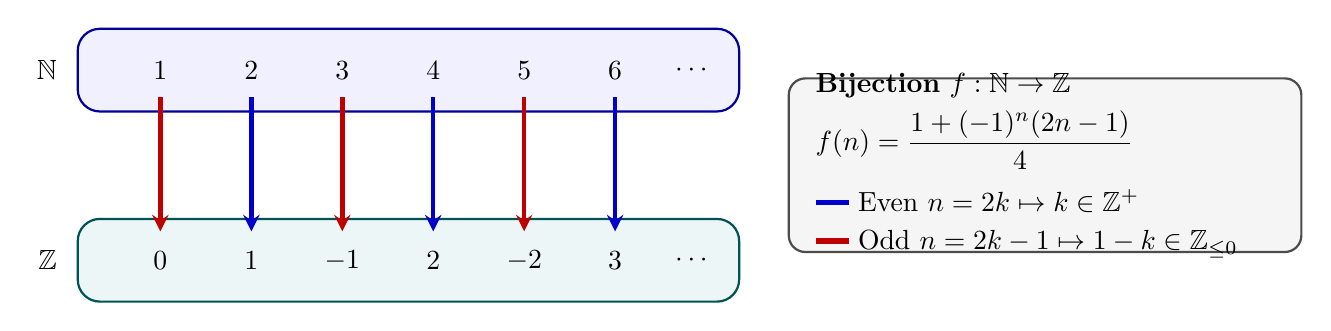
\begin{tikzpicture}[scale=1.05]
    % Layer 1: Background Shading
    \fill[blue!6, rounded corners=8pt] (-0.6, 1.75) rectangle (7.4, 2.75);
    \fill[teal!7, rounded corners=8pt] (-0.6, -0.55) rectangle (7.4, 0.45);
    \fill[gray!8, rounded corners=6pt] (8.0, 0.05) rectangle (14.2, 2.15);

    % Layer 2: Framing Borders / Set Boxes
    \draw[thick, blue!60!black, rounded corners=8pt] (-0.6, 1.75) rectangle (7.4, 2.75);
    \draw[thick, teal!65!black, rounded corners=8pt] (-0.6, -0.55) rectangle (7.4, 0.45);
    \draw[thick, gray!60!black, rounded corners=6pt] (8.0, 0.05) rectangle (14.2, 2.15);

    % Layer 3: Primary Mapping Arrows
    \foreach \x/\col in {0.4/red!75!black, 1.5/blue!80!black, 2.6/red!75!black, 3.7/blue!80!black, 4.8/red!75!black, 5.9/blue!80!black} {
        \draw[->, >=stealth, ultra thick, \col] (\x, 1.92) -- (\x, 0.30);
    }

    % Layer 4: Nodes and Labels
    \node[black, left=4pt] at (-0.6, 2.25) {$\displaystyle \mathbb{N}$};
    \node[black, left=4pt] at (-0.6, -0.05) {$\displaystyle \mathbb{Z}$};

    \foreach \x/\val in {0.4/1, 1.5/2, 2.6/3, 3.7/4, 4.8/5, 5.9/6} {
        \node[black] at (\x, 2.25) {$\displaystyle \val$};
    }
    \node[black] at (6.85, 2.25) {$\displaystyle \cdots$};

    \foreach \x/\val in {0.4/0, 1.5/1, 2.6/-1, 3.7/2, 4.8/-2, 5.9/3} {
        \node[black] at (\x, -0.05) {$\displaystyle \val$};
    }
    \node[black] at (6.85, -0.05) {$\displaystyle \cdots$};

    % Single-Node Multiline Legend anchored West in open margin
    \node[black, align=left, anchor=west, inner sep=8pt] at (8.05, 1.10) {
        \textbf{Bijection} $\displaystyle f : \mathbb{N} \to \mathbb{Z}$ \\[4pt]
        $\displaystyle f(n) = \frac{1 + (-1)^n (2n - 1)}{4}$ \\[6pt]
        {\color{blue!80!black}\rule[0.5ex]{1.2em}{2pt}} Even $n = 2k \mapsto k \in \mathbb{Z}^+$ \\[2pt]
        {\color{red!75!black}\rule[0.5ex]{1.2em}{2pt}} Odd $n = 2k - 1 \mapsto 1 - k \in \mathbb{Z}_{\le 0}$
    };
\end{tikzpicture}
\caption{Parity-interleaving bijection $f : \mathbb{N} \to \mathbb{Z}$ from Result 11.3 and Exercise 11.8. Disjoint parity classes map onto disjoint half-lines $\mathbb{Z}^+$ and $\mathbb{Z}_{\le 0}$, ensuring global injectivity and surjectivity.}
\end{figure}

\begin{figure}[htbp]
\centering
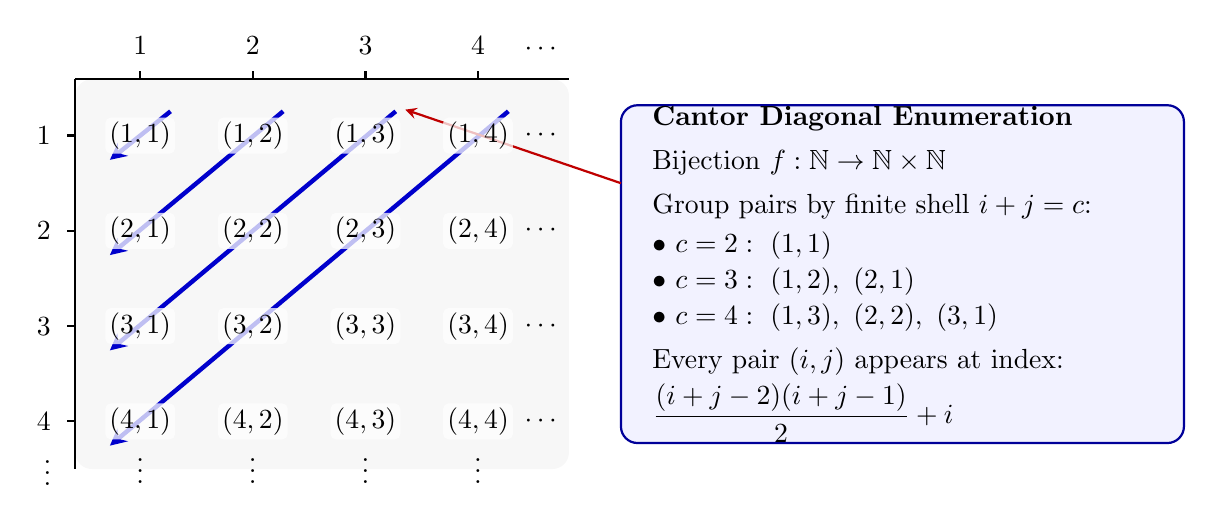
\begin{tikzpicture}[scale=1.1]
    % Layer 1: Background Shading
    \fill[gray!6, rounded corners=6pt] (0.55, 0.25) rectangle (6.25, 4.75);
    \fill[blue!5, rounded corners=6pt] (6.85, 0.55) rectangle (13.35, 4.45);

    % Layer 2: Grid Axes and Ticks
    \draw[thick, black] (0.55, 4.75) -- (6.25, 4.75);
    \draw[thick, black] (0.55, 4.75) -- (0.55, 0.25);
    \draw[thick, blue!60!black, rounded corners=6pt] (6.85, 0.55) rectangle (13.35, 4.45);

    \foreach \x/\col in {1.3/1, 2.6/2, 3.9/3, 5.2/4} {
        \draw[thick] (\x, 4.75) -- (\x, 4.85) node[black, above=2pt] {$\displaystyle \col$};
    }
    \node[black, above=2pt] at (5.95, 4.85) {$\displaystyle \cdots$};

    \foreach \y/\row in {4.1/1, 3.0/2, 1.9/3, 0.8/4} {
        \draw[thick] (0.55, \y) -- (0.45, \y) node[black, left=2pt] {$\displaystyle \row$};
    }
    \node[black, left=2pt] at (0.45, 0.30) {$\displaystyle \vdots$};

    % Layer 3: Primary Diagonal Traversal Arrows (Result 11.6)
    % Diagonal 1: (1,1)
    \draw[->, >=stealth, ultra thick, blue!80!black] (1.65, 4.38) -- (0.95, 3.82);
    % Diagonal 2: (1,2) -> (2,1)
    \draw[->, >=stealth, ultra thick, blue!80!black] (2.95, 4.38) -- (0.95, 2.72);
    % Diagonal 3: (1,3) -> (2,2) -> (3,1)
    \draw[->, >=stealth, ultra thick, blue!80!black] (4.25, 4.38) -- (0.95, 1.62);
    % Diagonal 4: (1,4) -> (2,3) -> (3,2) -> (4,1)
    \draw[->, >=stealth, ultra thick, blue!80!black] (5.55, 4.38) -- (0.95, 0.52);

    % Off-axis callout highlighting Diagonal c = 4
    \draw[->, >=stealth, shorten >=2pt, red!75!black, thick] (6.85, 3.55) -- (4.30, 4.42);

    % Layer 4: Grid Nodes and Legend
    \foreach \i/\y in {1/4.1, 2/3.0, 3/1.9, 4/0.8} {
        \foreach \j/\x in {1/1.3, 2/2.6, 3/3.9, 4/5.2} {
            \node[black, fill=white, fill opacity=0.75, text opacity=1, inner sep=1.5pt, rounded corners=2pt] at (\x, \y) {$\displaystyle (\i,\j)$};
        }
        \node[black] at (5.95, \y) {$\displaystyle \cdots$};
    }
    \foreach \x in {1.3, 2.6, 3.9, 5.2} {
        \node[black] at (\x, 0.32) {$\displaystyle \vdots$};
    }

    \node[black, align=left, anchor=west, inner sep=8pt] at (6.95, 2.50) {
        \textbf{Cantor Diagonal Enumeration} \\[4pt]
        Bijection $\displaystyle f : \mathbb{N} \to \mathbb{N} \times \mathbb{N}$ \\[4pt]
        Group pairs by finite shell $\displaystyle i + j = c$: \\[2pt]
        $\bullet\ c = 2:\ (1,1)$ \\[1pt]
        $\bullet\ c = 3:\ (1,2),\ (2,1)$ \\[1pt]
        $\bullet\ c = 4:\ (1,3),\ (2,2),\ (3,1)$ \\[4pt]
        Every pair $\displaystyle (i, j)$ appears at index: \\[2pt]
        $\displaystyle \frac{(i + j - 2)(i + j - 1)}{2} + i$
    };
\end{tikzpicture}
\caption{Cantor diagonal traversal of $\mathbb{N} \times \mathbb{N}$ (Result 11.6). Sweeping along finite anti-diagonals $i + j = c$ guarantees every ordered pair $(i, j)$ is visited in finitely many steps, unlike a row-by-row traversal.}
\end{figure}

\subsection{Heuristics and ``Cheats''}

\begin{itemize}
    \item \textbf{The Theorem 11.4 Shortcut:} Whenever asked to prove a set $S$ is denumerable and $S$ looks like a constrained subset of $\mathbb{N}$, $\mathbb{Z}$, $\mathbb{Q}$, or $\mathbb{N} \times \mathbb{N}$, immediately ask: \emph{``Can I just prove $S$ is infinite and invoke Theorem 11.4?''} This bypasses painful piecewise formulas in seconds (as in Exercises 11.12, 11.14, 11.15, and 11.17).
    \item \textbf{How to Prove a Set Is Infinite in Two Lines:} To show $S$ is infinite, exhibit an obvious injection $\phi : \mathbb{N} \to S$ (e.g., $k \mapsto (1, k)$ or $k \mapsto a_{k^2 + 1}$). A set containing a denumerable subset cannot be finite!
    \item \textbf{Parity Splitting vs.\ Prime-Power Packing:} Need to pack $2$ copies of $\mathbb{N}$ into $\mathbb{N}$? Use even and odd numbers ($2k, 2k-1$). Need to pack $m$ copies of $\mathbb{N}$ into $\mathbb{N}$? Use residue classes modulo $m$. Need to pack \emph{infinitely many} copies of $\mathbb{N}$ into $\mathbb{N}$? Use $2^{m-1}(2n - 1)$ (Exercise 11.18) or prime powers $p_m^n$.
    \item \textbf{Always Check Well-Definedness First:} Before proving injectivity or surjectivity of a formula like $f(n) = \frac{1 + (-1)^n(2n-1)}{4}$ or $f(x) = \frac{2x}{x-1}$, check that the denominator never vanishes and the output genuinely lands inside the declared codomain (e.g., $\mathbb{Z}$ or $\mathbb{R} - \{2\}$).
\end{itemize}

\subsection{Pitfalls and Logical Fallacies}

\begin{enumerate}[label=\textbf{\arabic*.}]
    \item \textbf{The Row-by-Row Enumeration Fallacy:} Attempting to list $\mathbb{N} \times \mathbb{N}$ or $\bigcup_{i=1}^{\infty} A_i$ by listing all of Row $1$ first, then Row $2$, is \emph{not} a bijection from $\mathbb{N}$. Because Row $1$ is infinite, no element of Row $2$ is ever assigned a finite natural number index $n \in \mathbb{N}$ (see Figure 11.6 of the text).
    \item \textbf{Forgetting Disjointness in Unions:} If $A$ and $B$ are denumerable but overlap ($A \cap B \neq \emptyset$), the alternating function $f(2k-1) = a_k$, $f(2k) = b_k$ is \emph{not injective}, because any shared element appears twice! (One must either skip duplicates or decompose $A \cup B = A \cup (B - A)$.)
    \item \textbf{Applying Theorem 11.4 Without Proving Infiniteness:} A subset of a denumerable set is \emph{countable}, not automatically denumerable! It could be finite (or empty). You must explicitly prove $B$ is infinite before invoking Theorem 11.4.
    \item \textbf{Assuming ``$B \subsetneq A \implies |B| < |A|$'':} This finite-set intuition fails completely for infinite sets. Removing one element (Exercise 11.5), half the elements (Result 11.5), or infinitely many elements $\{a_{n^2}\}$ (Exercise 11.17) does not reduce the cardinality of a denumerable set.
    \item \textbf{Ignoring Duplicate Representations in $\mathbb{Q}^+$:} In the fraction grid $j/i$, the rational number $1/2$ appears infinitely often as $1/2, 2/4, 3/6, \dots$. Mapping directly from $\mathbb{N} \times \mathbb{N}$ to $\mathbb{Q}^+$ via $(i, j) \mapsto j/i$ is surjective, \emph{not} injective. One must bypass previously visited values (Result 11.7) or restrict to reduced fractions $\gcd(i, j) = 1$.
\end{enumerate}

% ============================================================================
% PART 5: CONCEPTUAL SYNTHESIS AND THE BIG PICTURE
% ============================================================================
\section{Conceptual Synthesis and the ``Big Picture''}

\subsection{Thematic Connections}

The overarching theme uniting all results in Section 11.2 is \textbf{structural invariance under discrete algebraic operations via bijective equivalence}. Rather than treating infinity as an amorphous monolith, we characterize the smallest infinite cardinality ($|\mathbb{N}| = \aleph_0$) as an equivalence class of sets closed under an astonishingly broad suite of operations:
\begin{itemize}
    \item \emph{Subsetting (downward closure):} Every infinite subset stays in the class (Theorem 11.4).
    \item \emph{Finite and denumerable unions:} Combining $2$ or even $\aleph_0$ copies of denumerable sets never escapes the class (Exercises 11.3, 11.16).
    \item \emph{Finite Cartesian products:} Multiplying two discrete dimensions collapses back into one discrete dimension (Result 11.6, Exercise 11.18).
    \item \emph{Algebraic extensions:} Expanding $\mathbb{N}$ to $\mathbb{Z}$ (additive inverses), to $\mathbb{Q}$ (multiplicative inverses), or to $\mathcal{G} = \mathbb{Z}[i]$ (Gaussian integers) leaves cardinality invariant.
\end{itemize}
In algebraic terms, denumerability is the universal benchmark of \emph{sequential listability}: any set whose elements can be uniquely encoded by finite discrete tuples of integers remains within the orbit of $\mathbb{N}$.

\subsection{Forward and Backward Links}

\textbf{Backward Links (How Denumerable Sets Extend Prior Concepts):}
Denumerable sets synthesize three foundational pillars from earlier mathematics:
\begin{itemize}
    \item \emph{Functions and Equivalence Relations:} Cardinality equality $|A| = |B|$ elevates bijections from concrete computational maps to an equivalence relation partitioning the universe of sets.
    \item \emph{Mathematical Induction and Well-Ordering:} The proof of Theorem 11.4 demonstrates that the Well-Ordering Principle on $\mathbb{N}$ is not merely a number-theoretic curiosity---it is the exact mechanism allowing us to extract a canonical linear order on any infinite subset of an enumerated set.
    \item \emph{Elementary Number Theory:} Parity, coprimality (reduced fractions in $\mathbb{Q}^+$), and unique prime factorization (specifically the $2$-adic bijection $2^{m-1}(2n-1)$) act as arithmetic compression engines that fold multi-dimensional discrete grids into $\mathbb{N}$.
\end{itemize}

\textbf{Forward Links (Bedrock for Advanced Mathematics):}
Denumerability is an indispensable pillar of nearly every advanced mathematical discipline:
\begin{itemize}
    \item \emph{Uncountable Sets and Cantor's Hierarchy:} Understanding the limits of denumerable lists sets the stage for identifying sets that \emph{cannot} be sequentially enumerated (such as intervals of real numbers) and distinguishing discrete infinity ($\aleph_0$) from the continuum.
    \item \emph{Measure Theory and Kolmogorov's Probability Axioms:} A probability measure $\mathbb{P}$ on a $\sigma$-algebra $\mathcal{F}$ must satisfy \emph{countable additivity}: for pairwise disjoint events $\{A_i\}_{i=1}^{\infty} \subseteq \mathcal{F}$, $\mathbb{P}\left(\bigcup_{i=1}^{\infty} A_i\right) = \sum_{i=1}^{\infty} \mathbb{P}(A_i)$. Because $\mathbb{Q}$ is denumerable, its Lebesgue measure is $\lambda(\mathbb{Q}) = \sum_{n=1}^{\infty} \lambda(\{q_n\}) = \sum_{n=1}^{\infty} 0 = 0$, despite $\mathbb{Q}$ being dense in $\mathbb{R}$!
    \item \emph{Real Analysis and Topology (Separability):} Because $\mathbb{Q}$ is a denumerable dense subset of $\mathbb{R}$, $\mathbb{R}$ is a \emph{separable} metric space. Separability guarantees countable bases in Hilbert spaces ($L^2$ spaces), enabling Fourier series expansions and Karhunen--Lo\`eve decompositions of stochastic processes.
    \item \emph{Theoretical Computer Science and Computability:} Every computer program is a finite string over a finite alphabet, so the set of all possible algorithms (Turing machines) is denumerable. This single cardinality fact underlies the existence of uncomputable functions and the limits of formal logic.
\end{itemize}

% ============================================================================
% PART 6: ABSTRACT REAL-WORLD MODELING (AI, ML, & QUANT FINANCE)
% ============================================================================
\section{Abstract Real-World Modeling (AI, ML, and Quantitative Finance)}

\subsection{Concrete Advanced Scenarios}

\begin{enumerate}[label=\textbf{\arabic*.}]
    \item \textbf{Limit Order Books and Discrete-Tick Stochastic Control (Algorithmic Trading \& Quantitative Finance):}
    In modern electronic financial markets, asset prices do not move continuously; they live on a discrete tick grid $\mathcal{S}_{\delta} = \delta \mathbb{Z} = \{\delta k : k \in \mathbb{Z}\}$ where $\delta > 0$ is the minimum tick size (e.g., $\$0.01$). By Result 11.5, $\mathcal{S}_{\delta}$ is a denumerable state space. Similarly, the joint queue state of bid and ask depths across $M$ price levels lives in $\mathbb{N}_0^{2M}$ (a finite Cartesian product of countable sets, hence denumerable by induction on Result 11.6). Modeling order-book dynamics as a Continuous-Time Markov Chain (CTMC) on this denumerable state space relies directly on bijective indexing $f : \mathbb{N} \to \mathcal{S}$ to write the infinitesimal generator matrix $Q = (q_{ij})_{i,j \in \mathbb{N}}$, solve Kolmogorov's forward/backward equations, and optimize market-making policies via dynamic programming.

    \item \textbf{Countable Hypothesis Spaces and PAC Generalization Bounds (Statistical Learning Theory \& AI):}
    In machine learning, a neural network architecture with floating-point weights, or the set of all decision trees / symbolic programs over a finite vocabulary $\Sigma$, forms a \emph{denumerable hypothesis class} $\mathcal{H} = \{h_1, h_2, h_3, \dots\}$. Because $\mathcal{H}$ is denumerable, we can assign a convergent prior weight distribution $\{w_n\}_{n=1}^{\infty}$ with $w_n > 0$ and $\sum_{n=1}^{\infty} w_n = 1$ (for instance, $w_n = 2^{-n}$ or $w_n = \frac{6}{\pi^2 n^2}$). Applying the countable subadditivity of probability measures (the \emph{countable union bound}) over the denumerable index set $\mathbb{N}$ yields non-vacuous Occam's Razor / Structural Risk Minimization generalization bounds that hold simultaneously for \emph{all} infinitely many hypotheses $h_n \in \mathcal{H}$!

    \item \textbf{Compound Poisson Jump-Diffusion Pricing on Discrete Regimes (Stochastic Calculus \& Derivatives Pricing):}
    When pricing financial derivatives under sudden market crashes or discrete earnings surprises, the log-asset price follows a jump-diffusion process driven by Brownian motion plus a compound Poisson process whose jump sizes take values in a denumerable set of tick-aligned shocks $\mathcal{J} = \{y_k : k \in \mathbb{N}\} \subset \mathbb{R} - \{0\}$. Countable additivity over the denumerable jump-size support allows the L\'evy measure $\nu$ to be written as a purely atomic sum $\nu(dy) = \sum_{k=1}^{\infty} \lambda_k \delta_{y_k}(dy)$, converting the Partial Integro-Differential Equation (PIDE) for option pricing into an exact countable difference-differential equation.
\end{enumerate}

\subsection{Rigorous Model Problem Setup: Jump-Diffusion Asset Pricing and Structural Risk Minimization on a Denumerable Space}

We construct a rigorous quantitative finance model illustrating how denumerable sets, explicit bijections, and countable additivity govern a \textbf{Discrete-Shock Jump-Diffusion Derivative Pricing Model} with a countable regime/shock architecture.

\subsubsection{Filtered Probability Space and Denumerable Shock Support}

Let $(\Omega, \mathcal{F}, (\mathcal{F}_t)_{t \ge 0}, \mathbb{P})$ be a complete filtered probability space satisfying the usual conditions. Suppose an equity price process $(S_t)_{t \ge 0}$ trades in a market subject to both continuous diffusive fluctuations and sudden discrete institutional shocks whose log-returns take values on a uniform tick grid $\mathcal{J} = \delta \mathbb{Z} - \{0\}$, where $\delta > 0$ is the log-tick resolution.

By Result 11.3 and Exercise 11.5 (applied to removing $0$ instead of $2$), $\mathcal{J}$ is a \textbf{denumerable set}. Explicitly, using a slight shift of the bijection from Exercise 11.8, we index $\mathcal{J} = \{y_1, y_2, y_3, \dots\}$ via the bijection $\gamma : \mathbb{N} \to \mathcal{J}$ defined by
\[
\gamma(k) = \begin{cases}
\dfrac{k + 1}{2}\delta & \text{if } k \text{ is odd}, \\[6pt]
-\dfrac{k}{2}\delta & \text{if } k \text{ is even},
\end{cases}
\]
which enumerates $\mathcal{J} = \{\delta, -\delta, 2\delta, -2\delta, 3\delta, -3\delta, \dots\}$ with each shock size appearing exactly once.

\subsubsection{Stochastic Dynamics and Countable L\'evy Measure}

For each shock level $y_k = \gamma(k) \in \mathcal{J}$, let $N_t^{(k)}$ be an independent homogeneous Poisson process with arrival intensity $\lambda_k > 0$, such that the total jump arrival rate is finite:
\[
\Lambda = \sum_{k=1}^{\infty} \lambda_k < \infty, \qquad \text{and} \qquad \sum_{k=1}^{\infty} \lambda_k \bigl|e^{y_k} - 1\bigr| < \infty.
\]
Under the physical measure $\mathbb{P}$, the asset price $(S_t)_{t \ge 0}$ obeys the Stochastic Differential Equation (SDE):
\[
\frac{dS_t}{S_{t^-}} = \mu\, dt + \sigma\, dW_t + \sum_{k=1}^{\infty} \bigl(e^{y_k} - 1\bigr)\, dN_t^{(k)}, \qquad S_0 > 0,
\]
where $(W_t)_{t \ge 0}$ is a standard $(\mathcal{F}_t)$-Brownian motion independent of $\{N_t^{(k)}\}_{k \in \mathbb{N}}$, $\mu \in \mathbb{R}$ is the drift, and $\sigma > 0$ is the diffusive volatility. Notice that because $\mathcal{J}$ is denumerable, the jump component is rigorously expressed as a countable superposition of independent Poisson channels, with total L\'evy measure
\[
\nu(A) = \sum_{k : y_k \in A} \lambda_k = \sum_{k=1}^{\infty} \lambda_k \mathbf{1}_{A}(y_k), \qquad A \in \mathcal{B}(\mathbb{R} - \{0\}),
\]
whose countable additivity is guaranteed by the absolute convergence of $\sum_{k=1}^{\infty} \lambda_k$.

\subsubsection{It\^o's Lemma for Jump-Diffusions and Risk-Neutral Martingale Pricing}

Let $r \ge 0$ be the constant risk-free interest rate. Under an equivalent risk-neutral martingale measure $\mathbb{Q} \sim \mathbb{P}$ (chosen via an Esscher transform assigning risk-neutral intensities $\tilde{\lambda}_k > 0$ with $\sum_{k=1}^{\infty} \tilde{\lambda}_k |e^{y_k} - 1| < \infty$), the discounted asset price $e^{-rt} S_t$ must be a $\mathbb{Q}$-martingale. Writing the compensated Poisson processes $\tilde{N}_t^{(k)} = N_t^{(k)} - \tilde{\lambda}_k t$, the no-arbitrage drift restriction requires
\[
\frac{dS_t}{S_{t^-}} = \left(r - \sum_{k=1}^{\infty} \tilde{\lambda}_k (e^{y_k} - 1)\right) dt + \sigma\, dW_t^{\mathbb{Q}} + \sum_{k=1}^{\infty} (e^{y_k} - 1)\, dN_t^{(k)}.
\]
Consider a European contingent claim with terminal payoff $\Phi(S_T)$ at maturity $T > 0$ and price function $V(t, S) = \mathbb{E}^{\mathbb{Q}}\!\left[e^{-r(T-t)}\Phi(S_T) \mid S_t = S\right] \in C^{1,2}([0, T) \times (0, \infty))$. Applying It\^o's Lemma for jump-diffusions to $e^{-rt} V(t, S_t)$ gives
\begin{align*}
d\bigl(e^{-rt} V(t, S_t)\bigr)
&= e^{-rt} \left[ -rV + \frac{\partial V}{\partial t} + \left(r - \sum_{k=1}^{\infty} \tilde{\lambda}_k (e^{y_k} - 1)\right) S \frac{\partial V}{\partial S} + \frac{1}{2}\sigma^2 S^2 \frac{\partial^2 V}{\partial S^2} \right. \\
&\qquad\qquad \left. + \sum_{k=1}^{\infty} \tilde{\lambda}_k \bigl(V(t, S e^{y_k}) - V(t, S)\bigr) \right] dt + dM_t^{\mathbb{Q}},
\end{align*}
where $M_t^{\mathbb{Q}}$ is a local $\mathbb{Q}$-martingale. Setting the finite-variation drift term to zero yields the governing \textbf{Countable-Jump Pricing Equation}:
\[
\frac{\partial V}{\partial t} + \left(r - \sum_{k=1}^{\infty} \tilde{\lambda}_k (e^{y_k} - 1)\right) S \frac{\partial V}{\partial S} + \frac{1}{2}\sigma^2 S^2 \frac{\partial^2 V}{\partial S^2} + \sum_{k=1}^{\infty} \tilde{\lambda}_k \bigl(V(t, S e^{y_k}) - V(t, S)\bigr) - rV = 0,
\]
subject to the terminal condition $V(T, S) = \Phi(S)$.

\subsubsection{Optimization / Calibration Problem}

Given a finite set of observed market option prices $\{V^{\text{mkt}}_j\}_{j=1}^{M}$ and an exponential tail-decay parameterization on the denumerable grid $\mathcal{J}$ (e.g., $\tilde{\lambda}_k = \alpha_+ e^{-\beta_+ \gamma(k)}$ for odd $k$ and $\tilde{\lambda}_k = \alpha_- e^{\beta_- \gamma(k)}$ for even $k$, ensuring $\sum_{k=1}^{\infty} \tilde{\lambda}_k e^{y_k} < \infty$ whenever $\beta_+ > 1$), the quantitative analyst solves the regularized inverse calibration problem:
\[
\min_{\theta = (\sigma, \alpha_+, \beta_+, \alpha_-, \beta_-)} \left\{ \sum_{j=1}^{M} w_j \bigl(V_{\theta}(0, S_0; K_j, T_j) - V^{\text{mkt}}_j\bigr)^2 + \eta\, D_{\mathrm{KL}}\bigl(\tilde{\lambda}(\theta) \,\|\, \lambda^{\text{prior}}\bigr) \right\},
\]
subject to $\sigma > 0$, $\alpha_{\pm} > 0$, $\beta_+ > 1$, $\beta_- > 0$, where the discrete Kullback--Leibler divergence over the denumerable index set $\mathbb{N}$ is
\[
D_{\mathrm{KL}}(\tilde{\lambda} \,\|\, \lambda^{\text{prior}}) = \sum_{k=1}^{\infty} \left( \tilde{\lambda}_k \ln\frac{\tilde{\lambda}_k}{\lambda_k^{\text{prior}}} - \tilde{\lambda}_k + \lambda_k^{\text{prior}} \right).
\]
This formulation showcases how the denumerability of $\mathcal{J}$ directly enables exact series representations, martingale compensation, and convergent information-theoretic regularization.

% ============================================================================
% PART 7: COMMON VARIATIONS AND UNTESTED CONCEPTS
% ============================================================================
\section{Common Variations and Untested Concepts}

Several important theorems concerning denumerable sets commonly appear on advanced proofs exams but were not explicitly assigned in Exercises 11.3--11.19. We present and rigorously prove four essential extensions below.

\subsection{Variation 1: Finite Cartesian Products of Denumerable Sets}

Result 11.6 handles $A \times B$ (two sets), but exams routinely ask for $n$-fold Cartesian products $\mathbb{N}^n$ or $A_1 \times A_2 \times \cdots \times A_n$.

\begin{proposition}
For every $n \in \mathbb{N}$, if $A_1, A_2, \dots, A_n$ are denumerable sets, then the Cartesian product $A_1 \times A_2 \times \cdots \times A_n$ is denumerable.
\end{proposition}

\begin{proof}
We proceed by mathematical induction on $n \in \mathbb{N}$.
\begin{itemize}
    \item \emph{Base Case ($n = 1$):} The $1$-fold product is simply $A_1$, which is denumerable by hypothesis. (For $n = 2$, $A_1 \times A_2$ is denumerable by Result 11.6.)
    \item \emph{Inductive Step:} Assume for some $k \in \mathbb{N}$ that the Cartesian product of any $k$ denumerable sets is denumerable. Let $A_1, A_2, \dots, A_k, A_{k+1}$ be denumerable sets. Define $P_k = A_1 \times \cdots \times A_k$. By the inductive hypothesis, $P_k$ is denumerable. Define the natural re-association map
    \[
    \Phi : P_k \times A_{k+1} \to A_1 \times A_2 \times \cdots \times A_k \times A_{k+1}
    \]
    by $\Phi\bigl((a_1, \dots, a_k), a_{k+1}\bigr) = (a_1, \dots, a_k, a_{k+1})$. Clearly $\Phi$ is bijective by the definition of equality of ordered tuples. Since both $P_k$ and $A_{k+1}$ are denumerable, Result 11.6 implies $P_k \times A_{k+1}$ is denumerable. By transitivity of numerical equivalence, $A_1 \times \cdots \times A_{k+1}$ is denumerable.
\end{itemize}
By the Principle of Mathematical Induction, the result holds for all $n \in \mathbb{N}$.
\end{proof}

\subsection{Variation 2: Countable Union of Possibly Overlapping Countable Sets}

Exercise 11.16 required the sets $A_1, A_2, \dots$ to be \emph{pairwise disjoint} and \emph{denumerable}. In probability theory and real analysis, we almost always drop both restrictions.

\begin{theorem}
If $A_1, A_2, A_3, \dots$ is a denumerable collection of countable sets (not necessarily pairwise disjoint or infinite), then $U = \bigcup_{i=1}^{\infty} A_i$ is countable.
\end{theorem}

\begin{proof}
If $U = \emptyset$, then $U$ is finite and hence countable. Assume $U \neq \emptyset$. First, discard any empty sets from the family, or simply note that for each nonempty $A_i$, since $A_i$ is countable, there exists a \emph{surjective} function $g_i : \mathbb{N} \to A_i$ (if $A_i = \{x_1, \dots, x_m\}$ is finite, define $g_i(j) = x_j$ for $1 \le j \le m$ and $g_i(j) = x_m$ for $j > m$; if $A_i$ is denumerable, take any bijection $g_i : \mathbb{N} \to A_i$). If $A_i = \emptyset$, pick a fixed element $u_0 \in U$ and define $g_i(j) = u_0$ for all $j \in \mathbb{N}$.

Now define $H : \mathbb{N} \times \mathbb{N} \to U$ by $H(i, j) = g_i(j)$. Then $H$ is surjective: for every $x \in U$, $x \in A_i$ for some $i \in \mathbb{N}$, and since $g_i$ maps onto $A_i$, there exists $j \in \mathbb{N}$ with $H(i, j) = g_i(j) = x$.

Let $\phi : \mathbb{N} \to \mathbb{N} \times \mathbb{N}$ be a bijection (Result 11.6). Then $F = H \circ \phi : \mathbb{N} \to U$ is a surjection. To convert this surjection into an injection going the opposite way, define $\psi : U \to \mathbb{N}$ by
\[
\psi(x) = \min\{n \in \mathbb{N} : F(n) = x\}.
\]
For every $x \in U$, the preimage $\{n \in \mathbb{N} : F(n) = x\}$ is a nonempty subset of $\mathbb{N}$ (because $F$ is surjective), so by the Well-Ordering Principle, $\psi(x) \in \mathbb{N}$ is uniquely defined. Moreover, $\psi$ is injective: if $\psi(x_1) = \psi(x_2) = m$, then by definition of $\psi$, $x_1 = F(m) = x_2$.

Since $\psi : U \to \mathbb{N}$ is a one-to-one function from a nonempty set $U$ into the denumerable set $\mathbb{N}$, it follows directly from Exercise 11.11 that $U$ is countable.
\end{proof}

\subsection{Variation 3: The Set of All Finite Subsets of $\mathbb{N}$}

Exercise 11.12 proved that the set of $2$-element subsets of $\mathbb{N}$ is denumerable. Remarkably, the collection of \emph{all} finite subsets of $\mathbb{N}$ is still denumerable!

\begin{theorem}
Let $\mathcal{F}(\mathbb{N}) = \{X \subseteq \mathbb{N} : X \text{ is finite}\}$. Then $\mathcal{F}(\mathbb{N})$ is denumerable.
\end{theorem}

\begin{proof}
We construct an explicit bijection $\Phi : \mathcal{F}(\mathbb{N}) \to \mathbb{N} \cup \{0\}$ using binary (base-$2$) representations. Define
\[
\Phi(\emptyset) = 0, \qquad \text{and for nonempty } X \in \mathcal{F}(\mathbb{N}), \qquad \Phi(X) = \sum_{k \in X} 2^{k - 1}.
\]
Because $X$ is finite, the sum is a finite sum of distinct powers of $2$, so $\Phi(X) \in \mathbb{N} \cup \{0\}$ is well-defined. By the uniqueness and existence of the binary expansion of every nonnegative integer:
\begin{itemize}
    \item \emph{Injectivity:} Distinct finite subsets $X \neq Y$ correspond to nonnegative integers whose base-$2$ digit strings differ in at least one bit position, so $\Phi(X) \neq \Phi(Y)$.
    \item \emph{Surjectivity:} Every nonnegative integer $m \in \mathbb{N} \cup \{0\}$ has a binary expansion $m = \sum_{j=0}^{r} d_j 2^j$ with $d_j \in \{0, 1\}$. Letting $X = \{j + 1 : d_j = 1\}$, $X \in \mathcal{F}(\mathbb{N})$ satisfies $\Phi(X) = m$.
\end{itemize}
Thus $|\mathcal{F}(\mathbb{N})| = |\mathbb{N} \cup \{0\}|$. Since $n \mapsto n - 1$ is a bijection from $\mathbb{N}$ to $\mathbb{N} \cup \{0\}$, $|\mathbb{N} \cup \{0\}| = |\mathbb{N}|$. By transitivity, $|\mathcal{F}(\mathbb{N})| = |\mathbb{N}|$, so $\mathcal{F}(\mathbb{N})$ is denumerable.
\end{proof}

\subsection{Variation 4: The Set of All Polynomials with Integer Coefficients $\mathbb{Z}[x]$}

\begin{theorem}
The set $\mathbb{Z}[x]$ of all polynomials in one variable $x$ with integer coefficients is denumerable.
\end{theorem}

\begin{proof}
For each integer $d \ge 0$, let $P_d$ denote the set of polynomials in $\mathbb{Z}[x]$ of degree at most $d$:
\[
P_d = \{c_0 + c_1 x + \cdots + c_d x^d : c_0, c_1, \dots, c_d \in \mathbb{Z}\}.
\]
The map $(c_0, c_1, \dots, c_d) \mapsto c_0 + c_1 x + \cdots + c_d x^d$ is a bijection from $\mathbb{Z}^{d+1}$ onto $P_d$. Since $\mathbb{Z}$ is denumerable (Result 11.3), Variation 1 implies that $\mathbb{Z}^{d+1}$ is denumerable, and therefore $P_d$ is denumerable for every $d \ge 0$.

Now write $\mathbb{Z}[x] = \bigcup_{d=0}^{\infty} P_d$. By Variation 2 (re-indexing $i = d + 1 \in \mathbb{N}$), $\mathbb{Z}[x]$ is a countable union of countable sets, so $\mathbb{Z}[x]$ is countable. Finally, $\mathbb{Z}[x]$ is infinite because it contains the infinite set of constant polynomials $\{n : n \in \mathbb{N}\}$. Hence $\mathbb{Z}[x]$ is denumerable.
\end{proof}

% ============================================================================
% PART 8: ADVANCED DIAGNOSTIC TESTING: "FIND THE FLAW"
% ============================================================================
\section{Advanced Diagnostic Testing: ``Find the Flaw''}

Each of the five proofs below appears polished and convincing at first glance, yet each contains a single, subtle, critical mathematical or logical flaw. Act as the grader: locate the exact error, explain why it invalidates the proof, and formulate the correct logical resolution. Check your diagnosis against the Solution Key at the end.

\subsection{Flawed Proof 1: Row-by-Row Enumeration of $\mathbb{N} \times \mathbb{N}$}

\textbf{Claim:} The set $\mathbb{N} \times \mathbb{N}$ is denumerable.

\textbf{Purported Proof:} Arrange all elements of $\mathbb{N} \times \mathbb{N}$ in an infinite grid where row $i$ contains $(i, 1), (i, 2), (i, 3), \dots$. Define a listing $f : \mathbb{N} \to \mathbb{N} \times \mathbb{N}$ by first listing all elements of Row $1$ in order: $(1, 1), (1, 2), (1, 3), \dots$; once Row $1$ is completed, proceed to Row $2$: $(2, 1), (2, 2), (2, 3), \dots$; once Row $2$ is completed, proceed to Row $3$, and continue inductively through all rows $i \in \mathbb{N}$. Since every ordered pair $(i, j)$ appears in row $i$ and column $j$ exactly once, this list visits every element of $\mathbb{N} \times \mathbb{N}$ exactly once. Hence $f$ is bijective and $\mathbb{N} \times \mathbb{N}$ is denumerable. $\square$

\subsection{Flawed Proof 2: Proving a Union of Two Denumerable Sets Is Denumerable}

\textbf{Claim:} If $A$ and $B$ are any two denumerable sets, then $A \cup B$ is denumerable.

\textbf{Purported Proof:} Since $A$ and $B$ are denumerable, write $A = \{a_1, a_2, a_3, \dots\}$ and $B = \{b_1, b_2, b_3, \dots\}$ where $a_i \neq a_j$ and $b_i \neq b_j$ for $i \neq j$. Define $f : \mathbb{N} \to A \cup B$ by
\[
f(n) = \begin{cases}
a_{(n+1)/2} & \text{if } n \text{ is odd}, \\[4pt]
b_{n/2} & \text{if } n \text{ is even}.
\end{cases}
\]
Clearly every $x \in A \cup B$ satisfies either $x = a_k = f(2k-1)$ or $x = b_k = f(2k)$, so $f$ is surjective. To check injectivity, note that $f$ maps distinct odd indices to distinct elements of $A$ (since $a_i \neq a_j$ for $i \neq j$) and maps distinct even indices to distinct elements of $B$ (since $b_i \neq b_j$ for $i \neq j$). Therefore $f$ is bijective, so $A \cup B$ is denumerable. $\square$

\subsection{Flawed Proof 3: Direct Application of Theorem 11.4 to an Arbitrary Intersection}

\textbf{Claim:} Let $A$ and $B$ be denumerable sets. Define $S = \{a \in A : a \in B\} = A \cap B$. Then $S$ is denumerable.

\textbf{Purported Proof:} Since $A$ is denumerable and $S = A \cap B \subseteq A$, $S$ is a subset of a denumerable set. Furthermore, $A$ and $B$ are both infinite sets, and every element of $S$ belongs to both infinite sets $A$ and $B$. By Theorem 11.4, every subset of a denumerable set obtained from infinite sets is denumerable. Therefore $S$ is denumerable. $\square$

\subsection{Flawed Proof 4: Bijection Between $\mathbb{N} \times \mathbb{N}$ and $\mathbb{Q}^+$}

\textbf{Claim:} The set $\mathbb{Q}^+$ of positive rational numbers is denumerable.

\textbf{Purported Proof:} By Result 11.6, $\mathbb{N} \times \mathbb{N}$ is denumerable, so there exists a bijection $\phi : \mathbb{N} \to \mathbb{N} \times \mathbb{N}$. Define $g : \mathbb{N} \times \mathbb{N} \to \mathbb{Q}^+$ by $g(a, b) = \frac{a}{b}$. Since every positive rational number can be written as $\frac{a}{b}$ for some $a, b \in \mathbb{N}$, $g$ is onto. Moreover, if $(a_1, b_1) = (a_2, b_2)$, then $\frac{a_1}{b_1} = \frac{a_2}{b_2}$, so $g$ is well-defined. Therefore $g \circ \phi : \mathbb{N} \to \mathbb{Q}^+$ establishes that $|\mathbb{Q}^+| = |\mathbb{N}|$, proving $\mathbb{Q}^+$ is denumerable. $\square$

\subsection{Flawed Proof 5: Inductive Proof That an Infinite Cartesian Product $\mathbb{N}^{\mathbb{N}}$ Is Denumerable}

\textbf{Claim:} The set $\mathbb{N}^{\mathbb{N}}$ of all infinite sequences $(x_1, x_2, x_3, \dots)$ of natural numbers is denumerable.

\textbf{Purported Proof:} Let $P(n)$ be the statement ``$\mathbb{N}^n$ is denumerable.'' For $n = 1$, $\mathbb{N}^1 = \mathbb{N}$ is denumerable, so $P(1)$ holds. Assuming $P(k)$ holds, $\mathbb{N}^{k+1}$ is bijective with $\mathbb{N}^k \times \mathbb{N}$, which is denumerable by Result 11.6; hence $P(k+1)$ holds. By the Principle of Mathematical Induction, $P(n)$ holds for all $n \in \mathbb{N}$. Letting $n \to \infty$, we conclude that $\mathbb{N}^{\mathbb{N}}$ is denumerable. $\square$

\subsection{Solution Key for ``Find the Flaw''}

\begin{enumerate}[label=\textbf{Flaw \arabic*:}]
    \item \textbf{Failure to Reach Later Rows in Finite Steps (Ill-Defined / Non-Surjective Function on $\mathbb{N}$):} \\
    \emph{Why it fails:} The phrase ``once Row $1$ is completed, proceed to Row $2$'' is meaningless for a function with domain $\mathbb{N}$. Row $1$ has infinitely many elements, which already consume \emph{all} natural numbers $n \in \mathbb{N}$ via $f(n) = (1, n)$. There is no natural number $n \in \mathbb{N}$ mapped to $(2, 1)$! Thus the purported map is not onto $\mathbb{N} \times \mathbb{N}$. \\
    \emph{Correct resolution:} Traverse the grid along finite anti-diagonals $i + j = c$ ($c = 2, 3, 4, \dots$), as in Result 11.6, or use an explicit bijection such as $f^{-1}(m, n) = 2^{m-1}(2n - 1)$ (Exercise 11.18).

    \item \textbf{Missing Disjointness Assumption (Failure of Injectivity Across Parity Classes):} \\
    \emph{Why it fails:} Checking injectivity separately on odd inputs and on even inputs does \emph{not} prove global injectivity! You must also rule out $f(\text{odd}) = f(\text{even})$. Because $A$ and $B$ were \emph{not} assumed to be disjoint, there could exist $x \in A \cap B$, say $x = a_i = b_j$. Then $f(2i - 1) = a_i = b_j = f(2j)$ with $2i - 1 \neq 2j$, destroying injectivity. \\
    \emph{Correct resolution:} Note that $A \cup B = A \cup (B - A)$, where $A$ and $B - A$ are disjoint. Since $B - A \subseteq B$, $B - A$ is either finite or denumerable (Theorem 11.4). If $B - A$ is denumerable, apply Exercise 11.3 to $A$ and $B - A$. If $B - A = \{c_1, \dots, c_m\}$ is finite, list $A \cup B$ as $c_1, \dots, c_m, a_1, a_2, a_3, \dots$ (shifting indices of $A$ by $m$).

    \item \textbf{Misapplication of Theorem 11.4 (Intersection of Infinite Sets Need Not Be Infinite):} \\
    \emph{Why it fails:} Theorem 11.4 states that every \emph{infinite} subset of a denumerable set is denumerable. The claim itself is false! Two denumerable sets can have an empty or finite intersection: for example, $A = \{2k : k \in \mathbb{N}\}$ and $B = \{2k - 1 : k \in \mathbb{N}\}$ have $A \cap B = \emptyset$, while $A = \mathbb{N}$ and $B = \{1, -1, -2, -3, \dots\}$ have $A \cap B = \{1\}$. \\
    \emph{Correct resolution:} The true statement is that $A \cap B$ is \emph{countable} (either finite or denumerable). If $A \cap B$ is additionally known to be infinite, then Theorem 11.4 implies $A \cap B$ is denumerable.

    \item \textbf{Confusing Well-Definedness with Injectivity (Duplicate Fractions):} \\
    \emph{Why it fails:} The proof checked surjectivity and well-definedness (which is the converse of injectivity: $x_1 = x_2 \implies g(x_1) = g(x_2)$), completely omitting injectivity! In fact, $g(a, b) = a/b$ is \emph{not} injective: $g(1, 2) = \frac{1}{2} = \frac{2}{4} = g(2, 4)$, yet $(1, 2) \neq (2, 4)$. Consequently, $g \circ \phi$ is not a bijection. \\
    \emph{Correct resolution:} Either restrict the domain of $g$ to the infinite subset $R = \{(a, b) \in \mathbb{N} \times \mathbb{N} : \gcd(a, b) = 1\}$ (on which $g|_R : R \to \mathbb{Q}^+$ \emph{is} bijective, and $R$ is denumerable by Theorem 11.4), or apply the duplicate-skipping diagonal algorithm of Result 11.7.

    \item \textbf{Illegitimate ``Letting $n \to \infty$'' in Mathematical Induction:} \\
    \emph{Why it fails:} Mathematical induction proves $P(n)$ holds for every \emph{finite} natural number $n \in \mathbb{N}$; it says nothing whatsoever about an infinite limit object at ``$n = \infty$.'' The property of being denumerable is \emph{not} preserved under countably infinite Cartesian products (in fact, $\mathbb{N}^{\mathbb{N}}$ is uncountable, as is even $\{0, 1\}^{\mathbb{N}}$). \\
    \emph{Correct resolution:} The statement for all finite $n \in \mathbb{N}$ is valid (Variation 1 in Section 7.1), proving that $\mathbb{N}^n$ is denumerable for every $n \in \mathbb{N}$---and even that the union of all \emph{finite} tuples $\bigcup_{n=1}^{\infty} \mathbb{N}^n$ is denumerable. However, one must never extrapolate a finite-induction property to an infinite Cartesian product.
\end{enumerate}

\end{document}